


\documentclass[11pt]{article}

\usepackage[top=.8in, bottom=.6in, left=.56in, right=.45in, footskip=0pt,
paperheight=13.4in,paperwidth=9.25in]{geometry}




\newcommand{\Ldown}[1]{\hspace{-2pt}\raisebox{-1pt}{{%\fontfamily{lmhh}
\fontsize{14}{11}\selectfont{}{\textnormal{#1.}}}}\hspace{3pt}}


\newcommand{\semihr}[1]{{\textcolor{orange!60!black}{\hrule width #1}}}


\usepackage{xcolor}


\usepackage{xcolor}



%\input{commands}

\newcommand{\mdash}{---}
\newcommand{\q}[1]{``#1''}
\newcommand{\br}{

}

\newcommand{\raggedRightTitle}[1]{\br{}\begin{flushleft}\textbf{#1}\end{flushleft}}

%\newcommand{\visavis}{vis-\`a-vis}


%\input{ngml/ngml-setup-commands}
%\input{ngml/ngml-sdi-commands}
%\input{ngml/ngml-deco-commands}

%\AtEndDocument{\immediate\write18{cd /home/nlevisrael/gits/ntxh/wip-sebi/ar/code/cpp/qmake-console/projects/gtagml/ngml-sdi-console; ./run-with-args.sh /home/nlevisrael/gits/ntxh/wip-sebi/gtagml/ctg/gen/ctg/ctg.gt.tex /home/nlevisrael/gits/ntxh/wip-sebi/gtagml/ctg/gen/ctg/ctg.gt.sdi.ntxh /home/nlevisrael/gits/ntxh/wip-sebi/gtagml/ctg/gen/ctg/ctg.gt.sdi-prelatex.ntxh; cd -;}}



% pmml  arff  openannotation

\usepackage[T1]{fontenc}
\usepackage{tgtermes}

\usepackage[hang,flushmargin]{footmisc}

\usepackage{titlesec}

\titlespacing*{\section}
{0pt}{4ex plus 1ex minus .5ex}{.1ex plus .2ex}

%\usepackage{titlesec}

\titleformat{\section}
  {\normalfont\Large\bfseries}   % The style of the section title
  {}                             % a prefix
  {0pt}                          % How much space exists between the prefix and the title
  {} 


%\usepackage{mathptmx}

\usepackage{eso-pic}

\AddToShipoutPictureBG{%

\colorlet{redbl}{red!40!magenta}
\colorlet{yelbl}{yellow!60!magenta}

\colorlet{redblg}{redbl!30!black}

\ifnum\value{page}>66{
\AtTextLowerLeft{\raisebox{-21pt}{\hspace{-15pt}\fontfamily{qtm}\fontsize{10}{11}\fontseries{b}\selectfont{}{\colorbox{yelbl!7}{\textcolor{redblg!70}{PLEASE SEE OUR SOFTWARE DEMO VIDEOS: \href{http://www.lingtechsys.com/videos/qmt-composite.mkv}{GIS},
\href{http://www.lingtechsys.com/videos/dhax-composite.mkv}{360\textdegree{} photography}, and \href{http://www.lingtechsys.com/videos/xcsd-composite.mkv}{image processing}.}}}}}
}\fi
}


%\setlength\parindent{0pt}

\AddToShipoutPictureBG{%

\ifnum\value{page}>1{
\AtTextUpperLeft{
\makebox[23.1cm][r]{
\raisebox{-.6cm}{%
{\transparent{0.3}{
\includegraphics[width=0.19\textwidth]{e-logo.png}}	}} } }
}\fi
}

\AddToShipoutPicture{%
{
 {\color{blGreen!70!red}\transparent{0.9}{\put(0,0){\rule{3pt}{\paperheight}}}}%
 {\color{darkRed!70!purple}\transparent{1}\put(3,0){{\rule{4pt}{\paperheight}}}}
% {\color{logoPeach!80!cyan}\transparent{0.5}{\put(0,700){\rule{1cm}{.6cm}}}}%
% {\color{darkRed!60!cyan}\transparent{0.7}\put(0,706){{\rule{1cm}{.6cm}}}}
% \put(18,726){\thepage}
% \transparent{0.8}
}
}

%\AddToShipoutPicture{%
%\ifnum\value{page}=1
%\put(247.5,988){%
%	\transparent{0.7}{
%		\includegraphics[width=0.4\textwidth]{logo.png}}}
%\fi
%}	


\AddToShipoutPictureBG{%
\ifnum\value{page}=14

\put(7,678){
	\transparent{1}{
		\includegraphics[angle=0.5,origin=c,width=0.4\textwidth]{pm/1a.jpg}}}


\put(241,698){
	\transparent{1}{
		\includegraphics[angle=0,origin=c,width=0.31\textwidth,
trim=0 14mm 0 10mm, clip]{pm/7a.png}}}


\put(6,492){
	\transparent{1}{
		\includegraphics[angle=-0.5,origin=c,width=0.4\textwidth]{pm/5a.png}}}


\put(452,712){
	\transparent{1}{
		\includegraphics[angle=-1,origin=c,width=0.3\textwidth]{pm/2a.png}}}



\put(442,681){
	\transparent{1}{
		\includegraphics[angle=0,origin=c,width=0.18\textwidth]{pm/8a.png}}}


%\put(412,680){
%	\transparent{1}{
%		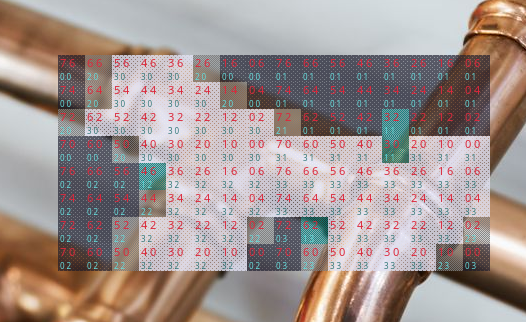
\includegraphics[angle=2.5,origin=c,width=0.2\textwidth]{pm/8.png}}}


\put(402,487){
	\transparent{1}{
		\includegraphics[angle=-1,origin=c,width=0.45\textwidth]{pm/3a.jpg}}}

\fi
}	




%\pagestyle{empty} % no page number
%\parskip 7.2pt    % space between paragraphs
%\parindent 12pt   % indent for new paragraph
%\textwidth 4.5in  % width of text
%\columnsep 0.8in  % separation between columns

%\setlength{\footskip}{-3pt}

%\usepackage[paperheight=15in,paperwidth=8.5in]{geometry}
%\geometry{left=.65in,top=.65in,right=.45in,bottom=1.25in} %margins

%\renewcommand{\thepage}{\raisebox{2pt}{\arabic{page}}}

\renewcommand{\footnoterule}{%
	\kern -3pt
	\hrule width .92\textwidth height .5pt
	\kern 10pt
}


\usepackage[hyphens]{url}
\newcommand{\biburl}[1]{ {\fontfamily{gar}\selectfont{\textcolor[rgb]{.2,.6,0}%
{\scriptsize {\url{#1}}}}}}

\newcommand{\bhref}[1]{\href{#1}{#1}}



%\linespread{1.3}

\newcommand{\sectsp}{\vspace{12pt}}

\usepackage{graphicx}
\usepackage{color,framed}

\usepackage{textcomp}

\usepackage{float}

\usepackage{mdframed}


\usepackage{setspace}

\usepackage{xcolor}

\usepackage[hyphenbreaks]{breakurl}
\usepackage[hyphens]{url}

%\usepackage{hyperref}

\colorlet{blCyan}{cyan!50!blue}

\definecolor{darkRed}{rgb}{.2,.0,.1}


\definecolor{blGreen}{rgb}{.2,.7,.3}

\definecolor{darkBlGreen}{rgb}{.1,.3,.2}

\definecolor{oldBlColor}{rgb}{.2,.7,.3}

\definecolor{blColor}{rgb}{.1,.3,.2}

\definecolor{elColor}{rgb}{.2,.1,0}
\definecolor{flColor}{rgb}{0.7,0.3,0.3}

\definecolor{logoOrange}{RGB}{108, 18, 30}
\definecolor{logoGreen}{RGB}{85, 153, 89}
\definecolor{logoPurple}{RGB}{200, 208, 30}

\definecolor{logoBlue}{RGB}{4, 2, 25}
\definecolor{logoPeach}{RGB}{255, 159, 102}
\definecolor{logoCyan}{RGB}{66, 206, 244}
\definecolor{logoRed}{rgb}{.3,0,0}

\newcommand{\colorq}[1]{{\color{logoOrange!70!black}{\q{\small\textbf{#1}}}}}

\let\qq\q

\definecolor{inOne}{rgb}{0.122, 0.435, 0.698}% Rule colour
\definecolor{inTwo}{rgb}{0.122, 0.698, 0.435}% Rule colour

\definecolor{outOne}{rgb}{0.435, 0.698, 0.122}% Rule colour
\definecolor{outTwo}{rgb}{0.698, 0.435, 0.122}% Rule colour

\colorlet{linkcolor}{flColor!60!red}




\usepackage[many]{tcolorbox}% http://ctan.org/pkg/tcolorbox

\usepackage{transparent}

\newlength{\bsep}
\setlength{\bsep}{-1pt}
\let\xbibitem\bibitem
\renewcommand{\bibitem}[2]{\vspace{\bsep}\xbibitem{#1}{#2}}

\newenvironment{cframed}{\begin{mdframed}[linecolor=logoPeach,linewidth=0.4mm]}{\end{mdframed}}

\newenvironment{ccframed}{\begin{mdframed}[backgroundcolor=logoGreen!5,linecolor=logoCyan!50!black,linewidth=0.4mm]}{\end{mdframed}}

\usepackage{aurical}
\usepackage[T1]{fontenc}

\usepackage{relsize}

\newcommand{\bref}[1]{\hspace*{1pt}\textbf{\ref{#1}}}

\newcommand{\dashsep}{--\hspace*{5pt}}

\newcommand{\pseudoIndent}{

\vspace{2pt}\hspace*{6pt}}

\usepackage{titlesec}

\titlespacing*{\subsection}
{0pt}{5ex plus 1ex minus .2ex}{0.5ex plus .2ex}


%\titlespacing*{\section}
%{0pt}{3.5ex plus 1ex minus .2ex}{1ex plus .2ex}

%
\newcommand{\deconum}[1]{{\protect\raisebox{-1pt}{{\LARGE #1}}}}

\newcommand{\visavis}{vis-\`a-vis}

\newcommand{\VersatileUX}{{\color{red!85!black}{\Fontauri Versatile}}%
{{\fontfamily{qhv}\selectfont\smaller UX}}}

\newcommand{\NDPCloud}{{\color{red!15!black}%
{\fontfamily{qhv}\selectfont {\smaller NDP C{\smaller LOUD}}}}}

\newcommand{\MThreeK}{{\color{blGreen!45!black}%
{\fontfamily{qhv}\fontsize{10}{8}\selectfont {M3K}}}}


\newcommand{\lfNDPCloud}{{\color{red!15!black}%
{\fontfamily{qhv}\selectfont N{\smaller DP C{\smaller LOUD}}}}}

\newcommand{\textds}[1]{{\fontfamily{lmdh}\selectfont{%
\raisebox{-1pt}{#1}}}}

\newcommand{\dsC}{{\textds{ds}{\fontfamily{qhv}\selectfont \raisebox{-1pt}
{\color{red!15!black}{C}}}}}

\definecolor{tcolor}{RGB}{24,52,61}

\newcommand{\CCpp}{\resizebox{!}{7pt}{\AcronymText{C}}/\Cpp{}}
\newcommand{\NoSQL}{\resizebox{!}{6.5pt}{\AcronymText{NoSQL}}}
\newcommand{\SQL}{\resizebox{!}{7pt}{\AcronymText{SQL}}}

\newcommand{\NCBI}{\resizebox{!}{7pt}{\AcronymText{NCBI}}}
\newcommand{\BioNetGen}{\resizebox{!}{7pt}{\AcronymText{BioNetGen}}}
\newcommand{\BNGL}{\resizebox{!}{7pt}{\AcronymText{BNGL}}}

\newcommand{\GML}{\resizebox{!}{7pt}{\AcronymText{GML}}}

\newcommand{\GIS}{\resizebox{!}{6.5pt}{\AcronymText{GIS}}}
\newcommand{\ACRIS}{\resizebox{!}{6.5pt}{\AcronymText{ACRIS}}}
\newcommand{\HPD}{\resizebox{!}{6.5pt}{\AcronymText{HPD}}}


\newcommand{\HTXN}{\resizebox{!}{7pt}{\AcronymText{HTXN}}}

\newcommand{\TDM}{\resizebox{!}{7pt}{\AcronymText{TDM}}}

\newcommand{\lHTXN}{\resizebox{!}{7.5pt}{\AcronymText{H}}%
\resizebox{!}{6.5pt}{\AcronymText{TXN}}}

\newcommand{\lsHTXN}{\resizebox{!}{9.5pt}{\AcronymText{\textcolor{tcolor}{HTXN}}}}

\newcommand{\LAF}{\resizebox{!}{7pt}{\AcronymText{LAF}}}

\newcommand{\UDpipe}{\resizebox{!}{7pt}{\AcronymText{UDpipe}}}

\newcommand{\C}{\resizebox{!}{7pt}{\AcronymText{C}}}

\newcommand{\TME}{\resizebox{!}{7pt}{\AcronymText{TME}}}

\newcommand{\TwoD}{\resizebox{!}{6.5pt}{\AcronymText{2D}}}




\usepackage{mdframed}

\newcommand{\cframedboxpanda}[1]{\begin{mdframed}[linecolor=yellow!70!blue,linewidth=0.4mm]#1\end{mdframed}}





\newcommand{\libSBML}{\resizebox{!}{7pt}{\AcronymText{libSBML}}}


\newcommand{\PVD}{\resizebox{!}{7pt}{\AcronymText{PVD}}}


\newcommand{\SDK}{\resizebox{!}{7pt}{\AcronymText{SDK}}}
\newcommand{\NLP}{\resizebox{!}{7pt}{\AcronymText{NLP}}}


\newcommand{\PDF}{\resizebox{!}{6.5pt}{\AcronymText{PDF}}}
\newcommand{\TEI}{\resizebox{!}{7.5pt}{\AcronymText{TE{\hspace*{.5pt}I}}}}
\newcommand{\SSML}{\resizebox{!}{7.5pt}{\AcronymText{SSML}}}
\newcommand{\ToBI}{\resizebox{!}{7.5pt}{\AcronymText{ToBI}}}

\newcommand{\MMBioS}{\resizebox{!}{6.5pt}{\AcronymText{MMBioS}}}

\newcommand{\VTK}{\resizebox{!}{6.5pt}{\AcronymText{VTK}}}


\newcommand{\AXF}{\resizebox{!}{7pt}{\AcronymText{AXF}}}

\newcommand{\HyperGraphDB}{\resizebox{!}{7pt}{\AcronymText{HyperGraphDB}}}


\newcommand{\lAXF}{\resizebox{!}{7.5pt}{\AcronymText{A}}%
\resizebox{!}{6.5pt}{\AcronymText{XF}}}


\newcommand{\lsAXF}{\resizebox{!}{8.5pt}{\AcronymText{AXF}}}

\newcommand{\AXFD}{\resizebox{!}{7pt}{\AcronymText{AXFD}}}

\newcommand{\lAXFD}{\resizebox{!}{7.5pt}{\AcronymText{A}}%
\resizebox{!}{6.5pt}{\AcronymText{XFD}}}


\newcommand{\IJST}{\resizebox{!}{7pt}{\AcronymText{IJST}}}

\newcommand{\BioC}{\resizebox{!}{7pt}{\AcronymText{BioC}}}

\newcommand{\CoNLL}{\resizebox{!}{7pt}{\AcronymText{CoNLL}}}
\newcommand{\CoNLLU}{\resizebox{!}{7pt}{\AcronymText{CoNLL-U}}}


\newcommand{\ePub}{\resizebox{!}{7pt}{\AcronymText{ePub}}}

%\lsLPF

\definecolor{atcColor}{RGB}{96, 17, 12}
%\textcolor{tcolor}{

\newcommand{\ATextCClr}[1]{\textcolor{atcColor}{\textbf{#1}}}

\newcommand{\ATexttclr}[1]{\textcolor{tcolor}{\textbf{#1}}}
\newcommand{\THQL}{\resizebox{!}{6.5pt}{\ATexttclr{THQL}}}


\newcommand{\ATextbk}[1]{\textcolor{black!50!cyan}{\textbf{#1}}}


%\newcommand{\lDHOS}{\resizebox{!}{7pt}{\ATexttclr{D}}%
%resizebox{!}{6.5pt}{\ATexttclr{HOS}}}

\newcommand{\PGVM}{\resizebox{!}{6.5pt}{\ATexttclr{PGVM}}}
\newcommand{\lPGVM}{\resizebox{!}{7pt}{\ATexttclr{PGVM}}}

\newcommand{\DHOS}{\resizebox{!}{6.5pt}{\ATexttclr{DHOS}}}
\newcommand{\lDHOS}{\resizebox{!}{7.5pt}{\ATexttclr{D}}\resizebox{!}{6.5pt}{\ATexttclr{HOS}}}
\newcommand{\sDHOS}{\resizebox{!}{6.5pt}{\ATexttclr{DHOS}}}

\newcommand{\sQt}{\resizebox{!}{6.5pt}{\ATexttclr{Qt}}}

\newcommand{\sPhVM}{\resizebox{!}{6.5pt}{\ATexttclr{P\hspace{.5pt}\textit{h}\hspace*{-.5pt}VM}}}


\newcommand{\PhVM}{\resizebox{!}{6.5pt}{\ATexttclr{P\hspace{.5pt}\textit{h}\hspace*{-.5pt}VM}}}
\newcommand{\lPhVM}{\resizebox{!}{7.5pt}{\ATexttclr{P}}\resizebox{!}{6.5pt}{\ATexttclr{\hspace{1pt}\textit{h}\hspace*{-.5pt}VM}}}


\newcommand{\MOC}{\resizebox{!}{7pt}{\AcronymText{MOC}}}
\newcommand{\SPARQL}{\resizebox{!}{7pt}{\AcronymText{SPARQL}}}
\newcommand{\GraphQL}{\resizebox{!}{7pt}{\AcronymText{GraphQL}}}

%{}, \QML{}, \GraphQL

\newcommand{\CCi}{\resizebox{!}{6.5pt}{\ATexttclr{CCi}}}
\newcommand{\XCSD}{\resizebox{!}{6.5pt}{\ATexttclr{XCSD}}}

\newcommand{\lXCSD}{\resizebox{!}{7pt}{\ATexttclr{XCSD}}}
\newcommand{\lCCi}{\resizebox{!}{7pt}{\ATexttclr{CCi}}}

%\newcommand{\ConceptsDB}{\resizebox{!}{6.5pt}{\ATexttclr{ConceptsDB}}}
%\newcommand{\lConceptsDB}{\resizebox{!}{7pt}{\ATexttclr{C}}\resizebox{!}{6.5pt}%{\ATexttclr{onceptsDB}}}


\newcommand{\GIT}{\resizebox{!}{7pt}{\AcronymText{GIT}}}

\newcommand{\LPF}{\resizebox{!}{7pt}{\AcronymText{LPF}}}
\newcommand{\lLPF}{\resizebox{!}{8.5pt}{\AcronymText{LPF}}}
\newcommand{\lsLPF}{\resizebox{!}{9.5pt}{\AcronymText{LPF}}}

\makeatletter

\newcommand*\getX[1]{\expandafter\getX@i#1\@nil}

\newcommand*\getY[1]{\expandafter\getY@i#1\@nil}
\def\getX@i#1,#2\@nil{#1}
\def\getY@i#1,#2\@nil{#2}
\makeatother
	
\newcommand{\rectann}[9]{%
\path [draw=#1,draw opacity=#2,line width=#3, fill=#4, fill opacity = #5, even odd rule] %
(#6) rectangle(\getX{#6}+#7,\getY{#6}+#8)
({\getX{#6}+((#7-(#7*#9))/2)},{\getY{#6}+((#8-(#8*#9))/2)}) rectangle %
({\getX{#6}+((#7-(#7*#9))/2)+#7*#9},{\getY{#6}+((#8-(#8*#9))/2)+#8*#9});}


\definecolor{pfcolor}{RGB}{94, 54, 73}

\newcommand{\EPF}{\resizebox{!}{7pt}{\AcronymText{ETS{\color{pfcolor}pf}}}}
\newcommand{\lEPF}{\resizebox{!}{8.5pt}{\AcronymText{ETS{\color{pfcolor}pf}}}}
\newcommand{\lsEPF}{\resizebox{!}{9.5pt}{\AcronymText{ETS{\color{pfcolor}pf}}}}

\newcommand{\RGB}{\resizebox{!}{6.5pt}{\AcronymText{RGB}}}


\newcommand{\GRE}{\resizebox{!}{7pt}{\AcronymText{GRE}}}
\newcommand{\CAS}{\resizebox{!}{7pt}{\AcronymText{CAS}}}

\newcommand{\lMOSAIC}{%
\resizebox{!}{8pt}{\AcronymText{M}}%
\resizebox{!}{6.5pt}{\AcronymText{OSAIC}}}

\newcommand{\XML}{\resizebox{!}{7pt}{\AcronymText{XML}}}
\newcommand{\RDF}{\resizebox{!}{7pt}{\AcronymText{RDF}}}
\newcommand{\DOM}{\resizebox{!}{7pt}{\AcronymText{DOM}}}


\newcommand{\CWL}{\resizebox{!}{7pt}{\AcronymText{CWL}}}




\newcommand{\Covid}{\resizebox{!}{7pt}{\AcronymText{Covid-19}}}

\newcommand{\CLang}{\resizebox{!}{7pt}{\AcronymText{C}}}

\newcommand{\HNaN}{\resizebox{!}{7pt}{\AcronymText{HN%
\textsc{a}N}}}

\newcommand{\JSON}{\resizebox{!}{7pt}{\AcronymText{JSON}}}

\newcommand{\MeshLab}{\resizebox{!}{7pt}{\AcronymText{MeshLab}}}
%\newcommand{\IQmol}{\resizebox{!}{7pt}{\AcronymText{IQmol}}}

\newcommand{\SGML}{\resizebox{!}{7pt}{\AcronymText{SGML}}}

\newcommand{\ASCII}{\resizebox{!}{7pt}{\AcronymText{ASCII}}}



\newcommand{\JATS}{\resizebox{!}{7pt}{\AcronymText{JATS}}}


\newcommand{\SDI}{\resizebox{!}{7pt}{\AcronymText{SDI}}}
\newcommand{\SDIV}{\resizebox{!}{7pt}{\AcronymText{SDIV}}}

\newcommand{\VXL}{\resizebox{!}{7pt}{\AcronymText{VXL}}}
\newcommand{\IQmol}{\resizebox{!}{7pt}{\AcronymText{IQmol}}}




\newcommand{\VM}{\resizebox{!}{7pt}{\AcronymText{VM}}}
\newcommand{\sVM}{\resizebox{!}{6.5pt}{\AcronymText{VM}}}


\newcommand{\IDE}{\resizebox{!}{7pt}{\AcronymText{IDE}}}


\newcommand{\OS}{\resizebox{!}{7pt}{\AcronymText{OS}}}

\newcommand{\FAIR}{\resizebox{!}{7pt}{\AcronymText{FAIR}}}
\newcommand{\FAIRsharing}{\resizebox{!}{7pt}{\AcronymText{FAIR}}\hspace*{1pt}\resizebox{!}{8pt}{sharing}}

\newcommand{\Python}{\resizebox{!}{7pt}{\AcronymText{Python}}}
\newcommand{\RPC}{\resizebox{!}{7pt}{\AcronymText{RPC}}}

\newcommand{\Java}{\resizebox{!}{7pt}{\AcronymText{Java}}}

\newcommand{\sBioNetGen}{\resizebox{!}{6.5pt}{\AcronymText{BioNetGen}}}
\newcommand{\sUI}{\resizebox{!}{6.5pt}{\AcronymText{UI}}}
\newcommand{\sAPOLLO}{\resizebox{!}{6.5pt}{\AcronymText{APOLLO}}}
\newcommand{\sSDK}{\resizebox{!}{6.5pt}{\AcronymText{SDK}}}
\newcommand{\sGUI}{\resizebox{!}{6.5pt}{\AcronymText{GUI}}}
\newcommand{\sAPI}{\resizebox{!}{6.5pt}{\AcronymText{API}}}




\newcommand{\QNetworkManager}{\resizebox{!}{7pt}{\AcronymText{QNetworkManager}}}
\newcommand{\QTextDocument}{\resizebox{!}{7pt}{\AcronymText{QTextDocument}}}

\newcommand{\QWebEngineView}{\resizebox{!}{6.5pt}{\AcronymText{QWebEngineView}}}

\newcommand{\HTTP}{\resizebox{!}{6.5pt}{\AcronymText{HTTP}}}


\newcommand{\lAcronymTextNC}[2]{{\fontfamily{fvs}\selectfont {\Large{#1}}{\large{#2}}}}

\newcommand{\AcronymTextNC}[1]{{\fontfamily{fvs}\selectfont {\large #1}}}



\colorlet{orr}{orange!60!red}

\colorlet{orb}{green!60!blue}
\colorlet{orbb}{green!30!blue}



\newcommand{\usstitle}[1]{\vspace{.4em}\raisebox{-1.2em}{{\fontfamily{gar}\fontsize{12}{14}%
\fontseries{sb}\selectfont{{\textcolor{orbb!65!black}{#1}}}}}}}


\newcommand{\sstitle}[1]{\vspace{1.4em}\raisebox{-1.2em}{{\fontfamily{gar}\fontsize{12}{14}%
\fontseries{sb}\selectfont{{\textcolor{orbb!65!black}{#1}}}}}}}

\newcommand{\DaSemio}{{\fontfamily{fvs}\fontsize{9}{14}%
\selectfont{\textbf{\textcolor{orb!75!black}{Da\resizebox{6pt}{!}{S}emio}}}}}}


\newcommand{\lDaSemio}{{\fontfamily{fvs}\fontsize{9}{14}%
\selectfont{\textbf{\textcolor{orb!75!black}{\resizebox{9pt}{!}{D}aSemio}}}}}}


%\newcommand{\DaSemio}{DaSemio}



\newcommand{\textscci}[1]{{\color{orr!35!black}{{%
						\fontfamily{Cabin-TLF}\fontseries{b}\selectfont{\textit{\scriptsize{#1}}}}}}}


\newcommand{\textscc}[1]{{\color{orr!35!black}{{%
						\fontfamily{Cabin-TLF}\fontseries{b}\selectfont{\textsc{\scriptsize{#1}}}}}}}


\newcommand{\textsccserif}[1]{{\color{orr!35!black}{{%
				\scriptsize{\textbf{#1}}}}}}


\newcommand{\iEPF}{\resizebox{!}{7pt}{\textsccserif{%
\textit{ETSpf}}}}

\newcommand{\iSDI}{\resizebox{!}{7pt}{\textsccserif{%
\textit{SDI}}}}

\newcommand{\iHTXN}{\resizebox{!}{7pt}{\textsccserif{%
\textit{HTXN}}}}




\newcommand{\AcronymText}[1]{{\textscc{#1}}}
\newcommand{\iAcronymText}[1]{{\textscci{#1}}}

\newcommand{\AcronymTextser}[1]{{\textsccserif{#1}}}


\newcommand{\mAcronymText}[1]{{\textscc{\normalsize{#1}}}}

\newcommand{\FASTA}{{\resizebox{!}{7pt}{\AcronymText{FASTA}}}}
\newcommand{\SRA}{{\resizebox{!}{7pt}{\AcronymText{SRA}}}}
\newcommand{\DNA}{{\resizebox{!}{7pt}{\AcronymText{DNA}}}}
\newcommand{\MAP}{{\resizebox{!}{7pt}{\AcronymText{MAP}}}}
\newcommand{\EPS}{{\resizebox{!}{7pt}{\AcronymText{EPS}}}}

\newcommand{\CSV}{{\resizebox{!}{6.5pt}{\AcronymText{CSV}}}}

%\newcommand{\PDB}{{\resizebox{!}{7pt}{\AcronymText{PDB}}}}


\newcommand{\APOLLO}{{\resizebox{!}{7pt}{\AcronymText{APOLLO}}}}
\newcommand{\GDC}{{\resizebox{!}{7pt}{\AcronymText{GDC}}}}
\newcommand{\TCIA}{{\resizebox{!}{7pt}{\AcronymText{TCIA}}}}
\newcommand{\CPTAC}{{\resizebox{!}{7pt}{\AcronymText{CPTAC}}}}





\newcommand{\XOCS}{{\resizebox{!}{7pt}{\AcronymText{XOCS}}}}


\newcommand{\cytoLib}{{\resizebox{!}{7pt}{\AcronymText{cytoLib}}}}
\newcommand{\CaPTk}{{\resizebox{!}{7pt}{\AcronymText{CaPTk}}}}
\newcommand{\DCMTK}{{\resizebox{!}{7pt}{\AcronymText{DCMTK}}}}
%\newcommand{\VM}{{\resizebox{!}{7pt}{\AcronymText{VM}}}}
\newcommand{\DSL}{{\resizebox{!}{7pt}{\AcronymText{DSL}}}}
\newcommand{\Paraview}{{\resizebox{!}{7pt}{\AcronymText{ParaView}}}}
\newcommand{\BFP}{{\resizebox{!}{7pt}{\AcronymText{BFP}}}}





\newcommand{\ChemXML}{{\resizebox{!}{7pt}{\AcronymText{ChemXML}}}}

\newcommand{\TeXMECS}{\resizebox{!}{7pt}{\AcronymText{TeXMECS}}}

% pmml  arff  openannotation

\newcommand{\PMML}{\resizebox{!}{7pt}{\AcronymText{PMML}}}
\newcommand{\ARFF}{\resizebox{!}{7pt}{\AcronymText{ARFF}}}
\newcommand{\IeXML}{\resizebox{!}{7pt}{\AcronymText{IeXML}}}


\newcommand{\NGML}{\resizebox{!}{7pt}{\AcronymText{NGML}}}


\newcommand{\WhiteDB}{\resizebox{!}{7pt}{\AcronymText{WhiteDB}}}

\colorlet{drp}{darkRed!70!purple}

%\newcommand{\MOSAIC}{{\color{drp}{\AcronymTextNC{\scriptsize{MOSAIC}}}}}

\newcommand{\MOSAIC}{\resizebox{!}{7pt}{\AcronymText{MOSAIC}}}


\newcommand{\mMOSAIC}{{\color{drp}{\AcronymTextNC{\normalsize{MOSAIC}}}}}

\newcommand{\MOSAICVM}{\mMOSAIC-\mAcronymText{VM}}

\newcommand{\sMOSAICVM}{\resizebox{!}{7pt}{\MOSAICVM}}
\newcommand{\sMOSAIC}{\resizebox{!}{7pt}{\MOSAIC}}

\newcommand{\LDOM}{\resizebox{!}{7pt}{\AcronymText{LDOM}}}
\newcommand{\Cnineteen}{\resizebox{!}{7pt}{\AcronymText{CORD-19}}}

\newcommand{\lCnineteen}{\resizebox{!}{7.5pt}{\AcronymText{CORD-19}}}


\newcommand{\MOL}{\resizebox{!}{7pt}{\AcronymText{MOL}}}

\newcommand{\ACL}{\resizebox{!}{7pt}{\AcronymText{ACL}}}

\newcommand{\LXCR}{\resizebox{!}{7pt}{\AcronymText{LXCR}}}
\newcommand{\lLXCR}{\resizebox{!}{8.5pt}{\AcronymText{LXCR}}}
\newcommand{\lsLXCR}{\resizebox{!}{9.5pt}{\AcronymText{LXCR}}}

%\newcommand{\lMOSAIC}{{\color{drp}{\lAcronymTextNC{M}{OSAIC}}}}
\newcommand{\lfMOSAIC}{\resizebox{!}{9pt}{{\color{drp}{\lAcronymTextNC{M}{OSAIC}}}}}

\newcommand{\Mosaic}{\resizebox{!}{7pt}{\MOSAIC}}
\newcommand{\MosaicPortal}{{\color{drp}{\AcronymTextNC{MOSAIC Portal}}}}

\newcommand{\RnD}{\resizebox{!}{7pt}{\AcronymText{R\&D}}}

\newcommand{\Cpp}{\resizebox{!}{6.5pt}{\AcronymText{C++}}}
\newcommand{\sRPC}{\resizebox{!}{6.5pt}{\AcronymText{RPC}}}



\newcommand{\JavaScript}{\resizebox{!}{6.5pt}{\AcronymText{JavaScript}}}


\newcommand{\Qt}{\resizebox{!}{6.5pt}{\AcronymText{Qt}}}


\newcommand{\DICOM}{\resizebox{!}{6.5pt}{\AcronymText{DICOM}}}
\newcommand{\TIFF}{\resizebox{!}{6.5pt}{\AcronymText{TIFF}}}


\newcommand{\WSI}{\resizebox{!}{7.5pt}{\AcronymText{WSI}}}

\newcommand{\ITK}{\resizebox{!}{6.5pt}{\AcronymText{ITK}}}

\newcommand{\medInria}{\resizebox{!}{7.5pt}{\AcronymText{medInria}}}

\newcommand{\OpenCV}{\resizebox{!}{6.5pt}{\AcronymText{OpenCV}}}
\newcommand{\CvMat}{\resizebox{!}{6.5pt}{\AcronymText{CvMat}}}

\newcommand{\MTA}{\resizebox{!}{6.5pt}{\AcronymText{MTA}}}

\newcommand{\XYZ}{\resizebox{!}{6.5pt}{\AcronymText{XYZ}}}
\newcommand{\ULURP}{\resizebox{!}{6.5pt}{\AcronymText{ULURP}}}

\newcommand{\CEQR}{\resizebox{!}{6.5pt}{\AcronymText{CEQR}}}


\newcommand{\SLD}{\resizebox{!}{6.5pt}{\AcronymText{SLD}}}
\newcommand{\FITS}{\resizebox{!}{6.5pt}{\AcronymText{FITS}}}

\newcommand{\REST}{\resizebox{!}{6.5pt}{\AcronymText{REST}}}

\newcommand{\LLVM}{\resizebox{!}{6.5pt}{\AcronymText{LLVM}}}
\newcommand{\JVM}{\resizebox{!}{6.5pt}{\AcronymText{JVM}}}

\newcommand{\TRI}{\resizebox{!}{6.5pt}{\AcronymText{TRI}}}

\newcommand{\PFAS}{\resizebox{!}{6.5pt}{\AcronymText{PFAS}}}
\newcommand{\EPA}{\resizebox{!}{6.5pt}{\AcronymText{EPA}}}




\newcommand{\lVM}{\resizebox{!}{7pt}{VM}}
\newcommand{\stGUI}{\resizebox{!}{7pt}{GUI}}

\newcommand{\HDFfive}{\resizebox{!}{6.5pt}{\AcronymText{HDF5}}}
\newcommand{\HDFfour}{\resizebox{!}{6.5pt}{\AcronymText{HDF4}}}


\newcommand{\HfiveIM}{\resizebox{!}{6.5pt}{\AcronymText{H5IM}}}


\newcommand{\HDF}{\resizebox{!}{6.5pt}{\AcronymText{HDF}}}
\newcommand{\CDF}{\resizebox{!}{6.5pt}{\AcronymText{CDF}}}
\newcommand{\netCDF}{\resizebox{!}{6.5pt}{\AcronymText{netCDF}}}

\newcommand{\QGIS}{\resizebox{!}{6.5pt}{\AcronymText{QGIS}}}


\newcommand{\QtSQL}{\resizebox{!}{6.5pt}{\AcronymText{QtSQL}}}


\newcommand{\R}{\resizebox{!}{6.5pt}{\AcronymText{R}}}

\newcommand{\SciXML}{\resizebox{!}{7pt}{\AcronymText{SciXML}}}



\newcommand{\lGRE}{\resizebox{!}{7.5pt}{\AcronymText{GRE}}}

\newcommand{\p}[1]{

\vspace*{.65em}#1}

\renewcommand{\q}[1]{{\fontfamily{phv}\selectfont ``}#1{\fontfamily{phv}\selectfont ''}} 

%\newcommand{\deconum}[1]{{\textcircled{#1}}}


\renewcommand{\thesection}{\protect\mbox{\deconum{\Roman{section}}}}
\renewcommand{\thesubsection}{\arabic{section}.\arabic{subsection}}

\newcommand{\llMOSAIC}{\mbox{{\LARGE MOSAIC}}}
%\newcommand{\lfMOSAIC}{\mbox{M\small{OSAIC}}}

\newcommand{\llMosaic}{\llMOSAIC}
\newcommand{\lMosaic}{\lMOSAIC}
\newcommand{\lfMosaic}{\lfMOSAIC}


\newcommand{\llWC}{\mbox{{\LARGE WhiteCharmDB}}}

\newcommand{\llwh}{\mbox{{\LARGE White}}}
\newcommand{\llch}{\mbox{{\LARGE CharmDB}}}

\usepackage{enumitem}

\usepackage{pifont}

\colorlet{dsl}{purple!20!brown}
\colorlet{dslr}{dsl!70!blue}

\newcommand{\itemSymbol}{{\textcolor{dslr}{\ding{70}}}}

\setlist[itemize]{%
  leftmargin=2pt,
  label={\colorbox{dsl!15}{\textcolor{dslr}{\ding{70}}}},
  topsep=6pt,
  itemsep=1.5pt,               % space between items
  %font={\bfseries\sffamily}, % set the label font
  font=\normalfont\bfseries\color{dslr!50!black}, % if colour is needed
}

\setlist[enumerate]{%
  leftmargin=10pt,
  topsep=7pt,               % space before start / after end of list
  itemsep=6pt,               % space between items
  font={\bfseries\sffamily}, % set the label font
%  font={\bfseries\sffamily\color{red}}, % if colour is needed
}

%\usepackage{tcolorbox}

\newcommand{\slead}[1]{%
\noindent{\raisebox{2pt}{\relscale{1.15}{{{%
\fcolorbox{logoCyan!50!black}{logoGreen!5}{#1}
}}}}}\hspace{.5em}}


\let\OldLaTeX\LaTeX

\renewcommand{\LaTeX}{\resizebox{!}{7pt}{\color{orr!35!black}{\OldLaTeX}}}

\let\OldTeX\TeX

\renewcommand{\TeX}{\resizebox{!}{7pt}{\color{orr!35!black}{\OldTeX}}}


\newcommand{\LargeLaTeX}{\resizebox{!}{8.5pt}{\color{orr!35!black}{\OldLaTeX}}}

\setlength\parindent{0pt}
%\setlength\parindent{24pt}
%\input{commands}


\newcommand{\lun}[1]{\raisebox{-4pt}{\fontfamily{phv}\selectfont{%
\LARGE{\textbf{\textcolor{tcolor}{#1}}}}}\vspace{-2pt}}

\newcommand{\inditem}{\itemindent10pt\item}



\newcommand{\LVee}{{\colorbox{cyan!40!yellow}{\textcolor{red!70!navy}{\textbf{\LARGE$\vee$}}}}}
\newcommand{\LWedge}{{\colorbox{cyan!40!yellow}{\textcolor{red!70!navy}{\textbf{\LARGE$\wedge$}}}}}


\newcommand{\ATxt}[1]{\AcronymText{#1}}

\usepackage{extdash}

%\newcommand{\ConceptsDB}{\resizebox{!}{7pt}{\ATexttclr{Concepts}\sDB}}
%\newcommand{\lConceptsDB}{\resizebox{!}{8pt}{\ATexttclr{C}}\resizebox{!}{6.5pt}{\ATexttclr{oncepts}\sDB}}}

\newcommand{\mScText}[1]{{\fontfamily{gar}\fontsize{10}{14}\selectfont{}#1}}
\newcommand{\mDB}{\mScText{\hspace{.5pt}D\hspace{-.5pt}B}}
\newcommand{\mConceptsDB}{\resizebox{!}{7.5pt}{\ATexttclr{Concepts}\mDB}}

\newcommand{\sConceptsDB}{\resizebox{!}{6.5pt}{\ATexttclr{Concepts}\sDB}}


\newcommand{\GIS}{\resizebox{!}{6.5pt}{\ATxt{GIS}}}
\newcommand{\AEC}{\resizebox{!}{6.5pt}{\ATxt{AEC}}}
\newcommand{\BIM}{\resizebox{!}{6.5pt}{\ATxt{BIM}}}
\newcommand{\IFC}{\resizebox{!}{6.5pt}{\ATxt{IFC}}}
\newcommand{\DSL}{\resizebox{!}{6.5pt}{\ATxt{DSL}}}
\newcommand{\API}{\resizebox{!}{6.5pt}{\ATxt{API}}}
\newcommand{\NoSQL}{\resizebox{!}{6.5pt}{\ATxt{NoSQL}}}

\newcommand{\ABI}{\resizebox{!}{6.5pt}{\ATxt{ABI}}}
\newcommand{\TSI}{\resizebox{!}{6.5pt}{\ATxt{TSI}}}

\newcommand{\PMH}{\resizebox{!}{6.5pt}{\ATxt{PMH}}}
\newcommand{\CAD}{\resizebox{!}{6.5pt}{\ATxt{CAD}}}

\newcommand{\MFC}{\resizebox{!}{6.5pt}{\ATxt{MFC}}}
\newcommand{\AWS}{\resizebox{!}{6.5pt}{\ATxt{AWS}}}

\newcommand{\NIEHS}{\resizebox{!}{6.5pt}{\ATxt{NIEHS}}}

\newcommand{\CORDNineteen}{\resizebox{!}{6.5pt}{\ATxt{CORD-19}}}

\newcommand{\dhref}[1]{\href{#1}{#1}}




\newcommand{\DWMS}{\resizebox{!}{6.5pt}{\ATxt{DWM\&S}}}
\newcommand{\OEM}{\resizebox{!}{6.5pt}{\ATxt{OEM}}}
\newcommand{\FEMA}{\resizebox{!}{6.5pt}{\ATxt{FEMA}}}
\newcommand{\PRISM}{\resizebox{!}{6.5pt}{\ATxt{PRISM}}}
\newcommand{\PRiSM}{\resizebox{!}{6.5pt}{\ATxt{PRiSM}}}

\newcommand{\ZoLa}{\resizebox{!}{6.5pt}{\ATxt{ZoLa}}}

\newcommand{\NJDEP}{\resizebox{!}{6.5pt}{\ATxt{NJ-DEP}}}

\newcommand{\HTML}{\resizebox{!}{6.5pt}{\AcronymText{HTML}}}

\newcommand{\PDB}{\resizebox{!}{6.5pt}{\ATxt{PDB}}}

\newcommand{\SDF}{\resizebox{!}{6.5pt}{\ATxt{SDF}}}

\newcommand{\AI}{\resizebox{!}{6.5pt}{\ATxt{AI}}}

\newcommand{\AItwo}{\resizebox{!}{6.5pt}{\ATxt{AI2}}}

\newcommand{\TRI}{{\resizebox{!}{6.5pt}{\AcronymText{TRI}}}}

\newcommand{\DfMA}{{\resizebox{!}{6.5pt}{\AcronymText{DfMA}}}}

\newcommand{\EXPRESS}{{\resizebox{!}{6.5pt}{\AcronymText{EXPRESS}}}}

\newcommand{\NASA}{{\resizebox{!}{6.5pt}{\AcronymText{NASA}}}}

\newcommand{\TIOBE}{{\resizebox{!}{6.5pt}{\AcronymText{TIOBE}}}}

\newcommand{\IPR}{{\resizebox{!}{6.5pt}{\AcronymText{IPR}}}}

\newcommand{\RVO}{{\resizebox{!}{6.5pt}{\AcronymText{RVO}}}}
\newcommand{\R}{{\resizebox{!}{6.5pt}{\AcronymText{R}}}}

\newcommand{\TMP}{{\resizebox{!}{6.5pt}{\AcronymText{TMP}}}}


\newcommand{\lTRI}{{\resizebox{!}{6.5pt}{\AcronymText{T}}}{\resizebox{!}{6.5pt}{\AcronymText{RI}}}}


\newcommand{\lTSI}{{\resizebox{!}{6.5pt}{\AcronymText{T}}}{\resizebox{!}{6.5pt}{\AcronymText{SI}}}}


\newcommand{\smbf}[1]{\resizebox{!}{6.5pt}{\textbf{#1}}}
\newcommand{\ssmbf}[1]{\resizebox{!}{5pt}{\textbf{#1}}}
\newcommand{\sssmbf}[1]{\resizebox{!}{4.75pt}{\textbf{#1}}}



\newcommand{\ArcGIS}{\smbf{Arc}\ssmbf{GIS}}



\newcommand{\iWRI}{\resizebox{!}{6.5pt}{\iAcronymText{WRI}}}
\newcommand{\iISI}{\resizebox{!}{6.5pt}{\iAcronymText{ISI}}}
\newcommand{\iAPI}{\resizebox{!}{6.5pt}{\iAcronymText{API}}}
\newcommand{\iACRIS}{\resizebox{!}{6.5pt}{\iAcronymText{ACRIS}}}
\newcommand{\iGIS}{\resizebox{!}{6.5pt}{\iAcronymText{GIS}}}



\newcommand{\visavis}{\resizebox{!}{6.5pt}{\ATxt{vis-`a-vis}}}


\newcommand{\WRI}{\resizebox{!}{6.5pt}{\ATxt{WRI}}}
\newcommand{\ISI}{\resizebox{!}{6.5pt}{\ATxt{ISI}}}
\newcommand{\ZCB}{\resizebox{!}{6.5pt}{\ATxt{ZCB}}}

\newcommand{\CEI}{\resizebox{!}{6.5pt}{\ATxt{CEI}}}
\newcommand{\TCP}{\resizebox{!}{6.5pt}{\ATxt{TCP}}}

\newcommand{\URL}{\resizebox{!}{6.5pt}{\ATxt{URL}}}


\newcommand{\CEOS}{\resizebox{!}{6.5pt}{\ATxt{CEOS}}}
\newcommand{\ODC}{\resizebox{!}{6.5pt}{\ATxt{ODC}}}
\newcommand{\HXL}{\resizebox{!}{6.5pt}{\ATxt{HXL}}}
\newcommand{\CHC}{\resizebox{!}{6.5pt}{\ATxt{CHC}}}
\newcommand{\WFP}{\resizebox{!}{6.5pt}{\ATxt{WFP}}}

\newcommand{\ZCB}{\resizebox{!}{6.5pt}{\ATxt{ZCB}}}


\newcommand{\IISD}{\resizebox{!}{6.5pt}{\ATxt{IISD}}}

\newcommand{\WRI}{\resizebox{!}{6.5pt}{\AcronymText{WRI}}}
\newcommand{\ISI}{\resizebox{!}{6.5pt}{\AcronymText{ISI}}}

\newcommand{\ThreeD}{\resizebox{!}{6.5pt}{\AcronymText{3D}}}
\newcommand{\TwoD}{\resizebox{!}{6.5pt}{\AcronymText{2D}}}


\newcommand{\GUI}{\resizebox{!}{6.5pt}{\AcronymText{GUI}}}
\newcommand{\UI}{\resizebox{!}{6.5pt}{\AcronymText{UI}}}

\usepackage{xcolor}


\definecolor{ulinkColor}{RGB}{47, 152, 196}
\definecolor{clinkColor}{RGB}{7, 152, 96}
\definecolor{alinkColor}{RGB}{147, 152, 46}


\usepackage[colorlinks = true,
            linkcolor = clinkColor,
            urlcolor  = clinkColor!70!purple,
            citecolor = clinkColor,
            anchorcolor = clinkColor]{hyperref}

\renewcommand{\thefootnote}{\textcolor{ulinkColor!50!black}{{\fontfamily{phv}\fontseries{b}\fontsize{7}{4}\selectfont\arabic{footnote}}}}



%\hypersetup{
%	colorlinks=true,
%	citecolor=blCyan!40!green,
%	filecolor=magenta!30!logoBlue,
%	urlcolor=blue,
%   linkcolor=linkcolor!70!black,
%    allcolors=blCyan!40!green
%}


\newcommand{\PPP}{\resizebox{!}{6.5pt}{\ATxt{PPP}}}
\newcommand{\SDK}{\resizebox{!}{6.5pt}{\ATxt{SDK}}}

\newcommand{\JPG}{\resizebox{!}{6.5pt}{\ATxt{JPG}}}
\newcommand{\SVG}{\resizebox{!}{6.5pt}{\ATxt{SVG}}}
\newcommand{\PNG}{\resizebox{!}{6.5pt}{\ATxt{PNG}}}


\newcommand{\mGIS}{\resizebox{!}{7pt}{\ATxt{GIS}}}
\newcommand{\mAEC}{\resizebox{!}{7pt}{\ATxt{AEC}}}
\newcommand{\mBIM}{\resizebox{!}{7pt}{\ATxt{BIM}}}
\newcommand{\mIFC}{\resizebox{!}{7pt}{\ATxt{IFC}}}
\newcommand{\mDSL}{\resizebox{!}{7pt}{\ATxt{DSL}}}
\newcommand{\mAPI}{\resizebox{!}{7pt}{\ATxt{API}}}
\newcommand{\mNoSQL}{\resizebox{!}{7pt}{\ATxt{NoSQL}}}

\newcommand{\sGIS}{\resizebox{!}{6.5pt}{\ATxt{GIS}}}
\newcommand{\sAPI}{\resizebox{!}{6.5pt}{\ATxt{AEC}}}
\newcommand{\sDSL}{\resizebox{!}{6.5pt}{\ATxt{DSL}}}



\renewcommand{\LVee}{}
\renewcommand{\LWedge}{}


\urlstyle{same}

\newcommand{\sectvspace}{\vspace{5pt}}


\usepackage{fnpct}

\newcommand{\curicon}[2]{%
	\node at (#1,#2) [
	draw=black,
	%minimum width=2ex,
	inner sep=.7pt,
	fill=white,
	single arrow,
	single arrow head extend=3pt,
	single arrow head indent=1.5pt,
	single arrow tip angle=45,
	line join=bevel,
	minimum height=4.6mm,
	rotate=115
	] {};
}




\renewcommand{\GIS}{\resizebox{!}{6pt}{\AcronymText{GIS}}}
\renewcommand{\VM}{\resizebox{!}{6pt}{\AcronymText{VM}}}
\renewcommand{\ABI}{\resizebox{!}{6pt}{\AcronymText{ABI}}}
\renewcommand{\Cpp}{\resizebox{!}{6pt}{\AcronymText{C++}}}
\renewcommand{\FAIR}{\resizebox{!}{6pt}{\AcronymText{FAIR}}}
\renewcommand{\FITS}{\resizebox{!}{6pt}{\AcronymText{FITS}}}
\renewcommand{\NASA}{\resizebox{!}{6pt}{\AcronymText{NASA}}}
\renewcommand{\ArcGIS}{\resizebox{!}{6pt}{\AcronymText{ArcGIS}}}
\renewcommand{\QFitsView}{\resizebox{!}{6pt}{\AcronymText{QFitsView}}}
\renewcommand{\PDF}{\resizebox{!}{6pt}{\AcronymText{PDF}}}
\renewcommand{\GUI}{\resizebox{!}{6pt}{\AcronymText{GUI}}}
\renewcommand{\ePub}{\resizebox{!}{6pt}{\AcronymText{ePub}}}

\renewcommand{\PFAS}{\resizebox{!}{6pt}{\AcronymText{PFAS}}}
\renewcommand{\QGIS}{\resizebox{!}{6pt}{\AcronymText{QGIS}}}
\renewcommand{\ThreeD}{\resizebox{!}{6pt}{\AcronymText{3D}}}

\renewcommand{\EPA}{\resizebox{!}{6pt}{\AcronymText{EPA}}}
\renewcommand{\TRI}{\resizebox{!}{6pt}{\AcronymText{TRI}}}

\renewcommand{\SarsCov}{\resizebox{!}{6pt}{\AcronymText{SARS-COV-2}}}

\renewcommand{\CAD}{\resizebox{!}{6pt}{\AcronymText{CAD}}}
\renewcommand{\XYZ}{\resizebox{!}{6pt}{\AcronymText{XYZ}}}

\renewcommand{\IQmol}{\resizebox{!}{6pt}{\AcronymText{IQmol}}}

\renewcommand{\FAIRsharing}{\resizebox{!}{6pt}{\AcronymText{FAIR}}\hspace*{1pt}\resizebox{!}{7pt}{sharing}}


\renewcommand{\lDaSemio}{{\fontfamily{fvs}\fontsize{8}{14}%
\selectfont{\textbf{\textcolor{orb!75!black}{\resizebox{8pt}{!}{D}aSemio}}}}}}






\usepackage{titleps}
\usepackage{tikz}
\usetikzlibrary{shapes}

\definecolor{AquaA5}{HTML}{4bacc6}
\definecolor{blggr}{rgb}{25, 180, 180}

\definecolor{rbl}{RGB}{225, 180, 180}

%\usepackage{soul}
\newcommand{\ul}[1]{\underline{#1}}

\newcommand*\fndiamondX[1]{\tikz[baseline=(char.base), x=2cm,y=1.5cm]{

 \node[shape=regular polygon, regular polygon sides=4, 
shape border rotate=45,
%shape=circle,
top color=red!31, bottom color=red!0,
inner sep=3pt, shading angle=210,xshift=.5pt] (char) at (0,0) {\ul{{#1}}};


 \node[shape=regular polygon, regular polygon sides=4, 
shape border rotate=45,
top color=AquaA5!50!black, bottom color=blggr!20,
inner sep=3pt, shading angle=210,xshift=.5pt] (char) at (0,5) {\ul{{#1}}};


}}


\newcommand*\fndiamond[1]{\tikz[baseline=(char.base)]{


% \node[shape=circle,fill=white,draw=white,
%inner sep=17pt, xshift=.5pt,yshift=-.5pt] (char) at (0,5) {};


 \node[shape=regular polygon, regular polygon sides=4, 
shape border rotate=45,
%shape=circle,
top color=rbl!30, bottom color=rbl!20,
inner sep=3pt, shading angle=210,xshift=.5pt] (char) at (0,0) {\ul{{#1}}};

 \node[shape=regular polygon, regular polygon sides=4, 
shape border rotate=45,
%shape=circle,
top color=AquaA5!50!black, bottom color=white,
inner sep=3pt, shading angle=210,xshift=.5pt] (char) at (0,0.15) {\ul{{#1}}};

 \node[shape=regular polygon, regular polygon sides=4, 
shape border rotate=45,
%shape=circle,
top color=AquaA5!50!black, bottom color=white,
inner sep=3pt, shading angle=210,xshift=.5pt] (char) at (0,0.2) {\ul{{#1}}};

 \node[shape=regular polygon, regular polygon sides=4, 
shape border rotate=45,
top color=white, bottom color=white,
fill opacity=1,
inner sep=2.5pt, shading angle=90,label={}] (bk)  at (0,0.2) {\ul{{#1}}};
%
}
}


\newcommand*\fnacircled[1]{\tikz[baseline=(char.base)]{

 \node[shape=regular polygon, regular polygon sides=5, 
shape border rotate=180,
%shape=circle,
top color=AquaA5!50!black, bottom color=blggr!20,
inner sep=4.5pt, shading angle=210,xshift=.5pt,yshift=-.5pt] (char) {\ul{#1}};

 \node[shape=regular polygon, regular polygon sides=5, 
shape border rotate=180,
top color=white, bottom color=blggr!20,
fill opacity=1,
inner sep=3.5pt, shading angle=90,label={}] (bk) {\ul{#1}};


% \node[shape=regular polygon,regular polygon sides=5,
%shape border rotate=180,
%AquaA5!50!black, bottom color=blggr!20, %top color=blggr!20, bottom color=yellow!20,
%inner sep=6pt, shading angle=125,xshift=.5pt,yshift=-.5pt,label={}] (char) {\ul{#1}};

% \node[shape=regular polygon,regular polygon sides=5,
%shape border rotate=180,
%fill opacity=1,top color=white, bottom color=blggr!20,
%inner sep=5.5pt, shading angle=90,label={}] (bk) {\ul{#1}};
}}









\newcommand*\fncircled[1]{\tikz[baseline=(char.base)]{

 \node[shape=circle,
top color=blggr!20, bottom color=AquaA5!90!black,
inner sep=7pt, shading angle=75,xshift=.5pt,yshift=-.5pt] (char) {\ul{#1}};

 \node[shape=circle,top color=white, bottom color=blggr!16,
fill opacity=1,
inner sep=6.5pt, shading angle=90,label={}] (bk) {\ul{#1}};
}}



\usepackage{fancyhdr} 
\pagestyle{fancy}


\fancypagestyle{lastpageX}{
    \renewcommand{\headrulewidth}{0pt}    
    \renewcommand{\footrulewidth}{0pt}
    \fancyfoot[C] {\fontsize{11}{11}\selectfont{\textcolor{logoOrange!50!magenta}{%
\fndiamond{\usepage}}}}}

}


\fancypagestyle{lastpage}{
    \renewcommand{\headrulewidth}{0pt}    
    \renewcommand{\footrulewidth}{0pt}

     \fancyfoot[C] {\hspace*{9pt}\fontsize{11}{11}\selectfont{\textcolor{logoOrange!50!magenta}{%
\fndiamond{\usepage}}}}

%     \fancyfoot[L] {\fontsize{11}{11}\selectfont{\textcolor{logoOrange!50!magenta}{%
%\fndiamondX{\usepage}}}}


%     \fancyfoot[C] {\fontsize{11}{11}\selectfont{\textcolor{logoOrange!50!magenta}{%
%\fndiamond{\usepage}}}}


%    \fancyfoot[C] {\fontsize{11}{11}\selectfont{\textcolor{logoOrange!50!magenta}{%
%\fndiamond{\usepage}}}}}
%    \fancyfoot[L] {\fontsize{11}{11}\selectfont{\textcolor{logoOrange!50!magenta}{%
%\fndiamondX{\usepage}}}

}


%\fontsize{11}{11}\selectfont{\textcolor{logoOrange!50!magenta}{%
%\fndiamond{\usepage}}}}

\fancypagestyle{firstpage}{
    \fancyhf{}
    \renewcommand{\headrulewidth}{0pt}    
    \renewcommand{\footrulewidth}{0pt}   
    \fancyfoot[C] {\fontsize{12}{11}\selectfont{\textcolor{logoOrange!50!magenta}{%
\fnacircled{\usepage}}}}}
}


\fancypagestyle{default}{
    \fancyhf{}           
    \renewcommand{\headrulewidth}{0pt}    
    \renewcommand{\footrulewidth}{0pt}   
    \fancyfoot[C] {\fontsize{12}{10}\selectfont{\textcolor{logoOrange!50!magenta}{%
\hspace{1.6em}\fncircled{\usepage}}}}}}
}


\fancypagestyle{predefault}{
    \fancyhf{}           
    \renewcommand{\headrulewidth}{0pt}    
    \renewcommand{\footrulewidth}{0.2pt}   
    \fancyfoot[RO, LE] {Pre \thepage}
}


\pagestyle{default}



%\begin{center}
%{\relscale{1.2}{\fontfamily{phv}\fontseries{b}\selectfont 
%{\colorbox{black}{\color{blue}{\llWC{} Database Engine \\and 
%\llMOSAIC{} Native Application Toolkit}}}}}

\colorlet{ctmp}{logoPeach!20!gray}
\colorlet{ctmpp}{ctmp!90!yellow}
\colorlet{ctmppp}{ctmpp!50!black}
\colorlet{ctmpppp}{ctmppp!90!logoRed}
\colorlet{ctmcyan}{ctmpppp!70!cyan}

\colorlet{ctmcyano}{ctmcyan!40!orange}
\colorlet{ctmcyanor}{ctmcyano!50!red}

\colorlet{cyann}{cyan!70!blue}

\newcommand{\cyanhr}{{\textcolor{cyann!40}{\hrule}}}

%109 52 4359

%\textcolor{logoRed}{\textbf{January 27, 2021}}

\newcommand{\sectprevspace}{\vspace{24pt}}

\newcommand{\sectnum}[1]{\hspace*{25pt}\textcolor{red!70!black}{}\hspace*{3pt}}

\newcommand{\secttitle}[1]{\textcolor{red!70!black}{\textit{\textbf{#1}}}}

\newcommand{\subtitle}[1]{\begin{center}\textcolor{purple!70!black}{\textit{\textbf{%
{\fontsize{11.5}{9.5}\selectfont{}#1}}}}\end{center}}

\newcommand{\cfootnote}[1]{\footnote{\centering #1}}


%\newcommand{\ConceptsDB}{\resizebox{!}{7.5pt}{\ATexttclr{ConceptsDB}}}

\newcommand{\lConceptsDB}{\resizebox{!}{7pt}{\ATexttclr{Concepts}}%
\resizebox{!}{6.5pt}{\ATexttclr{DB}}}

\newcommand{\llConceptsDB}{Concepts%
\hspace*{.5pt}\resizebox{!}{7.5pt}{\textcolor{dsl!70!black}{DB}}}

\newcommand{\PylonAthreeR}{\resizebox{!}{6.5pt}{\ATexttclr{Pylon}}%
\resizebox{!}{6pt}{\ATexttclr{A3R}}}


\newcommand{\lPylonAthreeR}{\resizebox{!}{7pt}{\ATexttclr{Pylon}}%
\resizebox{!}{6.5pt}{\ATexttclr{A3R}}}

\newcommand{\llPylonAthreeR}{Pylon%
\hspace*{.5pt}\resizebox{!}{7.5pt}{\textcolor{dsl!70!black}{A3R}}}


\newcommand{\PHCN}{\resizebox{!}{6.5pt}{\ATexttclr{PHCN}}}
\newcommand{\lPHCN}{\resizebox{!}{7pt}{\ATexttclr{P}}\resizebox{!}{6pt}{\ATexttclr{HCN}}}




\setlength{\itemsep}{10pt}


\AddToShipoutPictureBG{%

\colorlet{redbl}{red!40!magenta}
\colorlet{yelbl}{yellow!60!magenta}

\colorlet{redblg}{redbl!30!black}

%\ifnum\value{page}=5{
%\AtTextLowerLeft{\raisebox{-5pt}{\hspace{5pt}\fontfamily{qtm}\fontsize{10}{11}\fontseries{b}\selectfont{}{\colorbox{yelbl!7}{\textcolor{redblg!70}{PLEASE SEE OUR SOFTWARE DEMO VIDEOS: \href{http://www.lingtechsys.com/videos/qmt-composite.mkv}{GIS},
%\href{http://www.lingtechsys.com/videos/dhax-composite.mkv}{360\textdegree{} photography}, and \href{http://www.lingtechsys.com/videos/xcsd-composite.mkv}{image processing}.}}}}}
%}\fi


}




\begin{document}


%\setlength{\footskip}{22pt}


%\thispagestyle{empty}
\thispagestyle{firstpage}

\vspace*{90pt}

%\vspace*{1em}

\begin{center}

{\cyanhr}

\vspace*{11pt}

{\color{red!70!black}\fontfamily{phv}\fontseries{b}\selectfont

%\vspace*{13pt}

%{\Large{Solving the Machine Readable Problem}}

%\vspace*{10pt}

%{\Large{by}}

{\large{The Publishing Accelerator Toolkit (PacTk)}}

%\vspace*{7pt}

%{\large{as applied to Multimedia Government, Civil and Environmental Informatics}}

%\vspace*{7pt}

%{\large{Architecture, Construction, and Property Data}}

}

{\cyanhr}

\vspace*{55pt}

\hspace{-32pt}Amy Neustein, Ph.D.\\
\hspace{-32pt}CEO and Founder\\
\hspace{-32pt}Linguistic Technology Systems\\
\hspace{-32pt}Fort Lee, NJ\\
\hspace{-32pt}917-817-2184\\
\hspace{-32pt}\href{mailto://amy.neustein@verizon.net}{amy.neustein@verizon.net}

\end{center}

\vspace*{26pt}

%{\large{}}

%vspace*{6pt}


%}


\vspace*{12pt}

{\setstretch{1.12}


%\section{Overview}
%\vspace{}
\noindent\subtitle{{A Collection of Software, Compiler, and Runtime Tools \\
\vspace{4pt}
for Managing and Visualizing Multimedia Data Sets }}
%\sectvspace{}

\vspace*{-3pt}

\vspace*{10pt}
{\semihr{0.077\textwidth}}
\vspace*{3pt}
%\sectnum{1.}
\hspace{2pt}\secttitle{{Overview}}
\vspace*{5pt}
{\semihr{0.077\textwidth}}

\vspace*{3pt}

\p{In contemporary publishing, the standard workflow includes \XML{}-based 
formats such as \JATS{} or \BITS{} from which are compiled 
reader-visible documents such as \PDF{}s.  These intermediate 
files are distinct from those that authors submit directly, and they 
can be computationally accessed via generic \XML{}-oriented 
protocols such as \SAX{} (Simple \API{} for \XML{}), \XQuery{}, 
and \XQSE{} (\XQuery{} scripting extension).  Unfortunately, 
\XML{} itself is not explicitly built for representing 
textual data, and examining \JATS{} or \BITS{} files via 
generic \XML{} technology renders certain query and editing 
tasks difficult or impossible to implement.  The \PDF{} format 
is similarly opaque because internal \PDF{} representations 
of document text include many anomalies due to 
ligatures, hypenation, font specs, and other layout-related 
discrepancies between \XML{} inputs and user-visible output.}

\p{Given the limitataions of \XML{} for natural-language 
documents, numerous competing formats have been developed 
that provide alternatives or extensions to \XML{} structures, 
including \TEI{} (Text Encoding Initiative), \TagML{} 
(Text-as-Graph Markup Language), \BioC{} (a biomedical text mining 
standard defined by PubMed Central), and Research Object Bundles 
(a Semantic-Web based specification that convers both text and 
data sets).  With a proliferation of different text-encoding standards, 
query and traversal protocols that are developed for one specific 
format (e.g., \JATS{} and its derivatives) cannot be directly applied 
to others.  For example, the \XML{} parent-child element relationship 
is replaced in \TagML{} with two different containment styles 
(logical and extensional), such that \DOM{} and event-based 
parsers targeted at the simpler \XML{} hierarchy must be reimplemented 
for the \TagML{} system.  From the perspective of 
\PacTk{}, text-encoding evinces a spectrum of distinct 
\textit{topomorphic regimes} where a proliferation of 
incompatible document structures prohibits the emergence 
of common query, traversal, and metadata formats.}


\p{One important variation amongst text-encoding formats is 
the level of granularity for most textual elements.  In 
\JATS{}, \BITS{}, and most \JSON{} encodings, the fundamental 
discursive unit is the individual paragraph.  Elements on smaller 
scales (such as sentences or block quotes) are notated 
haphazardly at best.  \LaTeX{} employs reasonable 
sentence-boundary heuristics (that can be overriden via 
macros when necessary), but sentence objects are not expressed 
in any systematic manner (e.g., via auxiliary files) except 
for intermediate spacing.  In \TEI{} and \BioC{}, individual 
sentences \textit{can} be represented, but this is not 
mandatory (thus \textbf{s} and \textbf{sentence} tags 
are available but not guaranteed in any particular document).  
By contrast, \PacTk{} is explicitly built around 
sentence-level units, specifically a \q{topomorphic 
sentence-level object model} (\TSOM{}).  When all regular 
text in a natural-language document is explicitly 
contextualized in a delineated sentence object, many 
editing, indexing, and user-interface tasks become feasible 
(as outlined in the next section).}

\p{In contrast to the other formats mentioned here, 
\PacTk{} is not a single file format but rather a collection 
of code libaries and classes, with data types representing 
specific textual elements (sentences, paragraphs, \PDF{} pages, 
annotations and comment-boxes, etc.).  Query and traversal 
protocols modeled via \XQuery{}, \DOM{}, etc., become 
expressed by object methods and operators exposed to 
\Cpp{} code, for example (\PacTk{} is thus \q{topomorphic} 
in the sense that navigation between objects is determined 
by structural properties of divergent document formats, 
that manifest in competing notions of individuation for 
individual structure-sites and their interrelationships).  
In short, the \PacTk{} object system synthesizes distinct 
structuring protocols found in competing formats such as 
\JATS{}, \TagML{}, and \BioC{}, allowing publishers' workflows 
to inclduing each of these formats (and others) without 
sacrificing compatibility.  \lPacTk{} is particularly 
aimed at publishers who feel constrained by the limitations 
of \JATS{} or \BITS{} but are reluctant to try alternatives 
(\TagML{}, \BioC{}, etc.) due to minimal software-ecosystem support 
and the lack of standardized \XQuery{} and \DOM{}-style interfaces.} 
  
\p{The remainder of this document will discuss how 
\PacTk{} can streamline editing, indexing, and document-preparation 
tasks, as well as improve User Experience for human readers.  
Later sections will also address how \PacTk{} can contribute 
to broader projects where text documents are published together 
with data sets and/or multimedia presentations.}


\vspace*{10pt}
{\semihr{0.387\textwidth}}
\vspace*{5pt}
%\sectnum{1.}
\hspace{2pt}\secttitle{{Features for Editing, Indexing, and PDF Viewers}}
\vspace*{5pt}
{\semihr{0.387\textwidth}}

\vspace*{5pt}

  
\p{The computational foundation of \PacTk{} is the collection of 
classes that represented individual sentences and other 
textual elements in the \TSOM{} family (\PDF{} pages, annotations, 
footnotes, block quotes, edits or changes across document versions, etc.).  
In order to initialize these objects, \PacTk{} provides a distinct 
input format called \GTagML{}, or \q{grounded} \TagML{}.  
The term \q{grounded} reflects how certain structures-sites 
may be specifically marked as serializing a typed object: 
i.e., tags, attributes, or text nodes in the neighborhood 
of a site supply the data fields needed to initialize an 
object-instance during deserialization.  In other respects 
\GTagML{} follows most of the principles advocated by 
\TagML{}, with novel extensions; for example, \GTagML{} 
encourages the exploitation of Unicode Private Use Planes 
to disambiguate visibly similar but logically distinct characters/glyphs 
(e.g., periods may embody punctuation, acronyms, or abbreviations).  
In source files, \GTagML{} is loosely based on Markdown, so 
authors who use Markdown in more informal contexts 
(e.g., social media, chat rooms, \GIT{} documentation, etc.) 
will recognize many of the \GTagML{} styling commands.  
\lGTagML{} sources might be provided by authors directly, or 
derived from author inputs by digital copy editors or 
others on the publishing workflow.  To support 
\GTagML{}, \PacTk{} provides a new \Cpp{} parsing library 
that is readily extensible (more so than parsers for 
\XML{}, \JSON{}, and so forth), allowing publishers to 
customize the \GTagML{} format with new tags, syntax, and 
data structures specific to their in-house styles and 
disciplinary focus areas (e.g., specialized tags/data for 
different scientific fields --- chemistry, physics, medicine, 
etc. --- or whatever subject-areas are addressed by individual 
publishers, journals, and book series).  Alternatively, 
\TSOM{} objects can be compiled from sources such as 
\JATS{} or \BITS{} directly.}

\p{For workflows that feature \JATS{}, \BITS{}, or 
\LaTeX{}, \TSOM{} object bundles would be used as 
adjunct data sources through which edits, queries, 
and other computational artifacts would be routed.  
\lPacTk{} data can then be mapped both to 
archiving formats (like \XML{}) and camera-ready 
generators (like \LaTeX{}), but with a common 
\TSOM{} background these two different representational 
facets may be integrated (for example, \XML{} elements 
mapped to corresponding \PDF{} page coordinates).  
In effect, \PacTk{} serves to triangulate human-visible 
presentations (like \PDF{}) with behind-the-scenes 
\JATS{}-style formats.  Analyses that are currently 
implemented against \XML{} structures may be more 
efficiently coded via \PacTk{} objects, with concrete 
benefits in areas such as copy-editing and indexing.}



\sstitle{PacTk for Editing}

\p{In the case of \GIS{} data, digital mapping software such as 
\QGIS{} (to cite the most popular open-source application; \ArcGIS{}
is also widely used, but less amenable to third-party extensions)
enable users to visualize \GIS{} constructions --- especially  
regions and point-sets (taking specific locations as 
\textit{de facto} \q{points}) --- via formats such as 
shapefiles (\textbf{.shp}).  Attribute layers may then 
be superimposed employing formats such as \textbf{.sld} 
(Styled Layer Descriptor) to specify how visual cues 
should be rendered: in the case of mapping contaminants 
for hazard mitigation, the different pollutants tracked 
could be assigned distinct colors, and affected regions 
indicated via semi-transparent overlays.  Specific locations 
might be marked with icons whose appearance distinguishes 
different hazard categories (chemical leaks, fire, air 
pollution, harm to local ecosystems, public health concerns), 
perhaps evincing different sizes in accord with 
risk-assessment levels.  This kind of example typifies the 
overall strategy of \GIS{} User Interface design: color, 
size, iconography, and related visual conventions allow 
digital maps to be employed as summarial overviews of 
\GIS{} data sets.  However, such formats as \SLD{} 
do not support annotations for visual displays 
beyond the cartographic sketch; e.g., they do 
not proscribe how attribute data might be 
summarized in separate dedicated windows (like 
dialog boxes) or rendered as multimedia graphics.}

\p{In this context, the \DaSemio{} tools are intended to 
enable developers' formulation of data formats 
and protocols extending or replacing \SLD{} (and 
its analogs in other domains), allowing multimedia 
interop to be explicitly regulated via data-set 
materials.  In the case of environmental-hazard 
examples, \SLD{} files governing \GIS{} displays 
for contamination-related data sets could be 
augmented with stipulations for how chemical 
data would be visualized in software such as 
\IQmol{} --- that is, ensuring that users are presented 
with a consistent interface when loading molecular 
information into \IQmol{} based on the antecedent 
digital map-locations.  Similarly, multimedia applications such as 
video players could load annotations likewise stored 
in a data set; for instance, geotagging video frames 
would permit users to pause the video at a particular 
point and then, with interop enabled, have the 
map-display automatically scroll to the \GIS{} location 
presently visible on the video screen.  Video annotation 
might also superimpose text or graphics over segments 
of continuous frames, to more granularly relate the 
video content to the information tracked within the 
current data set.}

\p{For these scenarios, presentation 
formats such as \SLD{} must be significantly 
broadened in scope in order to recognize 
annotations and cross-application messaging 
spanning diverse media types.  Continuing the hypothetical 
environmental-hazards case study, a \QGIS{} user 
could visualize \GIS{} locations marked as 
contamination risks by loading data sets such as 
those archived under the Environmental Protection 
Agency's \q{Toxics Release Inventory} (\TRI{}) program.
To make the display useful, one then needs to 
superimpose some form of base map (e.g., 
Open Street Map tiles) and construct a style 
definition to regulate how data-set contents 
are cartographically iconified.  In principle, that 
could be achieved opening a style file, if one 
were available; often (as with \TRI{}) that is 
not the case, and even if so a truly effective display 
might require additional fine-tuning beyond  
static style declarations.}

\p{The preferred 
\QGIS{} approach in this case --- which is typical 
of many science applications --- is to automate and 
refine the data-set load process via Python scripts 
(or other embeddable languages, such as JavaScript).  
While supporting embeddable interpreters is 
important, choosing Python and other \q{general-purpose} 
scripting platforms introduces substantial added dependencies 
that complicate the software's build process and 
end-user operations.  From a developer's perspective, linking against 
platforms such as Python often demands juggling multiple 
installations and nontrivial build steps (these are not the 
sort of dependencies that can be encapsulated with a single 
\smbf{cmake} install-prefix line).  From an end-user's 
perspective, the host software has to coordinate with an 
external package manager insofar as scripts have their 
own dependencies, and it is frequently impossible to 
resolve coding errors or versioning conflicts within the 
application itself.}

\p{These are the sorts of problems we propose to address via 
embedded Virtual Machines (as outlined in the next section), 
which enable a fully-operational 
scripting platform to be embedded in applications without 
any external dependencies at all, simply by adding a 
suite of source-code files to the host-application project.}


\sstitle{Lacunae}

\p{In sum, we have reviewed a handful of technical challenges 
associated with multimedia data sets.  As a rule, current 
applications and data formats have not been implemented 
with multimedia interop as a important feature, 
so very few software or code libraries have been 
designed with relevant capabilities in mind.  
This is why we believe a package of extension and plugin libraries 
is necessary, to instantiate the sort of cross-application 
ecosystem allowing users to access and reuse multimedia 
data sets in a consistent and intuitive manner.}

\p{So as to build up that ecosystem, \DaSemio{} introduces 
components largely organized into three groups: 
compiler tools, multimedia cross-referencing, and 
ingredients for modular software aggregation 
(particularly \GUI{}s for individual multimedia 
content-types; also libraries involving 
database architecture and peer-to-peer cloud/native hosting). 
These are outlined respectively in the following sections.}



\vspace*{10pt}
{\semihr{0.387\textwidth}}
\vspace*{5pt}
%\sectnum{1.}
\hspace{2pt}\secttitle{{Compiler and Virtual Machine (\lVM) Components}}
\vspace*{5pt}
{\semihr{0.387\textwidth}}

\vspace*{5pt}


\p{Most \DaSemio{} components address concerns related to data sharing/integration.  Problems in this domain tend to fit into several categories: 1) data sets are typically shared in compacted formats that must be deserialized or decoded to become available for application users; 2) application and \GUI{} state should evolve to reflect the information structure of individual data sets; and 3) in contemporary science, data sets are considered to be distinct publications that 
(ideally) are cited and annotated by analogy to text documents --- not only referencing published data holistically but also granular parts or metadata contained therein.  Anyone working in scientific publishing over the past dozen or so years will have noted that publishing houses, as well as organizations that fund/sponsor academic research, have in that period prioritized data transparency and research replication: authors are encouraged (or required) to provide access to data sets and experiment results in conjunction with research articles.  Summarizing lab and/or data-acquisition protocols is also recommended, to facilitate others' double-checking research results and/or reproducing and generalizing/extending those results in alternate settings.  Yet the technological infrastructure for data publication has not evolved in step with data-transparency paradigms.  As a consequence, open-data repositories are populated with large numbers of weakly-curated resources which fail to meet standards such as \FAIRsharing{} (Findable, Accessible, Interoperable, Reusable), insofar as \q{raw data} is not intrinsically accessible, reusable, or interoperable.}


\p{Exacerbating this problem, scientists and publishers often lack a technical understanding of how data sets are loaded and processed, which results in confusion about how \FAIR{} protocols should be implemented in practice.  For instance, it is not uncommon for authors to conflate data sets themselves with summarial or analytic presentations, such as charts/plots or statistical breakdowns.  While there is nothing wrong with diagramming data-set statistics via inline tables or figures, open-data initiatives stipulate that data sets in their entirety should \textit{also} be published as separate entities.  When it comes to structuring complete data sets that \textit{are} published as integral wholes, another tendency is to assume that data publications become \q{reusable} insofar as they are assembled in compliance with popular standards, such as domain-specific protocols enforced by \RDF{} Ontologies or \XML{} Document-Type Declarations.  In reality, those forms of structural validators may guarantee that traversal algorithms proceed (and terminate) correctly, but such algorithms must still be implemented.  This is \q{Problem 1} listed above: users' access to data sets through science-oriented software entails reading individual values/records by decoding the data sets' elements into application-level datatype instances; here, Ontologies are useful but not sufficient for reconstituting data sets in live memory.  This problem is exacerbated in the context of specialized formats associated with specific scientific disciplines --- for instance, \CDF{} (Common Data Format) and \FITS{} (Flexible Image Transport System) in astronomy and Earth sciences --- which require dedicated parsers and/or binary stream consumers.  Even with generic formats such as \XML{} or \JSON{}, specialized computer code is still necessary in order to visit document nodes individually, reading each atomic value for assembly into aggregate structures.  In short, data sets must be \q{loaded} into research software in order to examine or manipulate them, which can only happen if software libraries are employed (or implemented) to parse and/or navigate around published information, as converted to traversable structures.}


\p{Since it is impractical for every science application to build parsers \textit{de novo}, organizations often spearhead the deployment and standardization of code libraries specifically associated with individual file types; \NASA{}'s repositories for \FITS{} media are a good example (in some cases, such as \CDF{} or \HDFfive{} --- the current \q{Hierarchical Data Format} --- standardized libraries are the \textit{only} way to access resources; elsewhere, re-implementing deserialization algorithms is possible in theory but infeasible in practice).  To preserve \FAIR{} standards, such libraries should be actively maintained, ported to multiple Operating Systems, and packaged for a wide variety of computing environments, particularly ones most associated with scientific research (Python, \R{}, \Qt{}, Java, etc.).  Yet publishers and research institutions often fail to coordinate the continued development and maintenance of data-sharing resources.  For example, publishers often list \q{Supplemental Materials} or \q{Data Availability} links alongside article abstracts, but they do not track the availability of software components equipped to read the specific formats adopted by those accessory data sets.  Also, a familiar complaint with general-purpose formats such as \netCDF{} and \HDFfive{} is that similar data sets are often encoded differently, so that application code (even when built on top of deserialization libraries) has to be rewritten for multiple (otherwise compatible) information sources; midstream \q{adapter} code is often not publicly accessible.  Nor are text formats such as \PDF{} or \ePub{} joined to (de)serialization libraries so that scientific papers could be cross-referenced with data sets and multimedia content on a granular level, based on annotations keyed to individual technical terms/acronyms, sentences, or paragraphs, rather than at the coarser scale of entire documents (Problem 3 above).  Similar comments could be made with respect to government agencies and other organizations charged with sharing civic, infrastructural (in the sense of Computer-Aided Design and Civil Engineering Informatics), or environmental data for public benefit.  In effect, publishers as well as research and governmental communities have failed to appreciate the distinct technological challenges associated with open data sharing in civil and/or scientific contexts.}


\sstitle{The Role of Compiler Technology in Data Sharing}

\p{In light of these difficulties, our solutions involve a dedicated Virtual Machine and Compiler Infrastructure specifically optimized for data sharing and modeling --- in other words, the foundation of a technology stack designed intrinsically around open-data requirements, rather than trying to fit transparency initiatives into (for example) generic web-programming paradigms.  To our knowledge, our work constitutes the only project which approaches the data-integration problem space from the perspective of compiler theory and \VM{} engineering.  The basic idea is to employ a largely self-contained \VM{} component which could be dropped in to code projects (including in source-code fashion) with few external dependencies.   Source libraries for parsing and navigating within domain-specific data formats can then be developed in code that compiles to this specific form of \VM{}, and thereby made available to any software which loads or links against the \VM{} as an embedded component or plugin.  Updates to data network/deserialization libraries are henceforth handled by the \VM{} in isolation from the host application.  This approach significantly reduces the overhead of porting and maintaining data-sharing code: because the \VM{} is largely autonomous \visavis{} its host environment, any library updates propagate automatically across \OS{} and computing platforms.}


\p{(We assume that projects are canonically implemented in \Cpp{}, since most scientific software is written in \Cpp{} and most of the rest can load \Cpp{} libraries. The definitive metric for language \q{popularity} and influence is the \TIOBE{} index, and the combination of \C{} and \Cpp{}, which is reasonable because most applications link against a mixture of both \C{} and \Cpp{} libraries, represents over 20\% percent of all existing computer code --- far above all other languages apart from Python at 15\% --- and collectively \Cpp{}, \C{}, and Python measure equally to all other top-20 languages combined; if we consider that Python is typically used as \q{glue} code delegating to native C/\Cpp{} libraries behind the scenes, it should be clear that the foundation of scientific computing is still, as much as ever, native-compiled components whose source languages are \C{} and \Cpp{} in some combination).}


\p{Embeddable \VM{}s provide a flexible infrastructure for coordinating simulations via automated workflows; an intermediary for database queries (via special instructions and/or foreign-function interface calls to emit a particular database engines' native query language); a fallback for binary data exchange when one or both endpoints do not link against (and can not dynamically load) compatible libraries/plugins to read/write the desired format; or a scripting basis for data-acquisition tasks.  In the latter case, applications could use scripts against data-provider \API{}s in lieu of users manually visiting web portals, which can be very cumbersone and involve multiple separate steps.  As another use case, consider Reference Implementations for specs which rely on constructions that are not natively supported by most programming languages (design-by-contract, measurement-unit annotations, certain forms of inter-type relationships, etc.).  Even languages primarily designed for compiling to native code could benefit from a \VM{} environment for prototyping grammar and semantics, most forms of testing (at least those not affected by variations in execution speed), and as a fallback option when source code does not build on a particular computer (due to, for instance, outdated system libraries; \smbf{glib}, say).  \VM{}s can also bridge multiple components for interop within foreign-function interface scenarios that must resolve such details as \Cpp{} name mangling.  Popular languages for science-related-code, like Python and \R{}, by contrast, often present significant difficulties when it comes to integration with native-compiled code libraries 
--- especially components such as \GUI{}s that employ frequent cross-module message passing.  An encouraging development is the emergence of new languages (e.g., \Cpp{} dialects like cppfront, Carbon, jank, Zig, and Circle) that directly generate and link against native libraries, while 
also introducing advanced design-by-contract and memory-management capabilities (among other innovations) --- although a richer compiler infrastructure could help these divergent projects cohere into a single \Cpp{} successor/extension framework (even if it has multiple top-level languages with different flavors, rather like the \JVM{}); we can imagine, for instance, the Stroustrup/dos Reis Internal Program Representation (\IPR{}) approach extending to \Cpp{} \q{successor} dialects.  Here, too, embedded \VM{}s are potentially valuable because they would permit variegated front languages to produce shared bytecode, without the overhead of a framework like \LLVM{} which, once it becomes a forced dependency, may significantly complicate an application's build process.}


\p{Another rationale for \VM{}-based implementations (even for languages that compile to native code) is to clarify compile-vs-runtime and template metaprogramming (\TMP{}) details.  Insofar as \VM{}s and the compilers that generate their code may both be seamlessly embedded in applications, it is possible to expose compilation \q{hooks} able to call arbitrary \Cpp{} functions (for example) and manipulate \VM{} bytecode directly --- a level of transparency that is not feasible when generating native machine code instead.  In several books we have discussed certain kinds of \q{back-door} communication between caller and callee procedures in terms of \q{channels,} which when properly utilized can enable many new runtime and static-analysis features (we also submitted a brief demo on the \q{\Cpp{} insights} website: \bhref{https://cppinsights.io/s/512c2700}).  There is some precedent for such techniques in existing \Cpp{} conventions, such as copy-elision and \q{Return Value Optimization} (\RVO{}) through which (in effect) procedures share (partial) access to their caller's stack frame.  One motivation for our own \VM{} implementation is to model augmented \RVO{} as a solution to existing \Cpp{} memory-management complications, related to extending temporary value lifetimes (proposed \q{lifetime annotations} import ideas from Rust into \Cpp{}, but we propose a more flexible method to achieve similar safety guarantees --- there's a brief summary on cppinsights at \bhref{https://cppinsights.io/s/cac923c9}).  The main point here is that \RVO{} represents one example of optimizations which can be modeled via what we call \q{channel algebra.}  It would be useful to free up such constructions so that compilers could extend \VM{} code with other channel-based features in a relatively open-ended manner.  Obviously, translating such models over to \Cpp{} compilers proper would require careful standardization (\RVO{} is supported only in a systematically enumerated set of circumstances, for example), but this is consistent with the general theme of prototyping language extensions in a \VM{} context and then investigating how and whether they are implementable for a \q{core} language in a compiler-neutral and cross-platform manner.}


\p{A Compiler/\VM{} infrastructure dedicated to data modeling and sharing has additional benefits, because it permits introducing features specifically oriented toward issues of data integrity and \FAIR{} protocols.  For example, specialized \VM{} instructions could be provided for dimensional analysis, measurement units, range limits, shape constraints, \q{axis-labeled} types (e.g., distinguishing number-pairs whose coordinates are \ssmbf{x}/\ssmbf{y} versus \sssmbf{row}/\smbf{column}, \smbf{width}/\smbf{height}, 
\smbf{first}/\smbf{second}, etc.), and other metadata details addressing the semantic integrity --- above and beyond syntactic propriety --- of individual fields/records.  Apart from validation, such semantic constructs serve as documentation and pedagogical tools for the scientific models and theories illustrated via data publications.  Also, \VM{}s provide a framework for scientific applications to expose their capabilities and user-visible state adaptably as data sets are loaded (Problem 2 above): individual data sets will often have information profiles that require special \GUI{} formulations or analytic processing within the host application.  Because data sets and digital models are not just static assertions of collected data points, but rather should function in effect as code libraries --- with dynamic simulation and/or project-specific interaction and visualization features --- models/sets should be engineered in environments which facilitate interop with scientific computing and advanced \UI{} libraries.  For instance, many image formats incorporate embedded metadata (\FITS{} data units, \TIFF{} tags, \DICOM{} attributes, etc.), so applications require --- in addition to the obvious graphics-display features --- some mechanism to show users content from metadata fields, at least insofar as those parameters are intrinsic components of the information being shared (and not behind-the-scenes specs expected to remain invisible, such as color-depth descriptions instructing software how to render image rasters).  Embedded \VM{}s allow applications to run scripts published alongside data sets, which would dynamically build \GUI{} windows or components, support domain-specific analyzers or workflows, and potentially expose certain parts of the overall application state (e.g., the toplevel window menubar; context menus; networking capabilities; or local filesystem access).}



\p{Interoperability across different scientific domains is limited because each discipline tends to have its own information-sharing ecosystem, often with decades-old roots, reflecting successive generations' favored theories about optimal data storage and processing.  Formats emerging during the heydey of 90s-era Object Databases often reflect certain modeling assumptions, that were to a nontrivial extent displaced by the Semantic Web fashion of the 2000s, only to see \q{Ontology} schemas decline in popularity against 2010s analytics and machine learning.  New tools and paradigms progressively complicate the goal of data interoperability, leading to new standards (often backwards-incompatible) which require new code libraries (cf., \HDFfive{} versus \HDFfour{}) and even a degree of convergence between formerly incompatible formats (cf., \HDFfive{} versus \netCDF{}).  These evolutionary trends present opportunities for data-management libraries to adapt and widen in scope, but institutions have to take the corresponding initiative.  Advances in data formats often correlate with innovations in software engineering and tooling, so larger technological factors can potentially be a catalyst for institutional re-prioritization of data-sharing capabilities.  For example, the Biden Administration recently (on February 26, 2024) released a \q{Statements of Support for Software Measurability and Memory Safety} that has garnered a lot of commentary in the computer science community; and may portend a (further) entrenchment of concepts such as lifetime annotations and software metrics among developers of programming-language toolsets.  On technical grounds it would be appropriate for these concerns to be explicitly addressed by future versions of libraries supporting formats such as \netCDF{} and \HDF{} (or their successors); see the above discussion about design-by-contract for concrete examples.}



\sstitle{Constraint Declarations and Other VM Use-Cases}

\p{Meanwhile, at least some information formats imply or presuppose the ability to represent computational procedures as components \textit{of} a data set (as opposed to tools for working \textit{with} a data set).  
For example, general-purpose modeling languages such as \EXPRESS{} sometimes support constraint declarations as intrinsic features of schemas, e.g., for defining derived types (wherein one type refines another via boolean predicates, restricting its domain).  Constraint-expressions may, at least sometimes and in theory, be notated via data structures built from primitive true/false tests such as equality and greater/less; however, it is arguably more accurate to treat constraints as subroutines behaviorally modeled via a reasonably expressive procedural language, one whose semantics would be consistent with general-purpose programming languages.  For instance, influential \EXPRESS{}-based standards, such as Industry Foundation Classes (\IFC{}) in engineering, require support for \q{procedural} data exchange (constituting \q{level 4} interoperability in the \IFC{} context) to ensure, above and beyond raw data duplication, that multiple components accessing a particular data set are able to transform it in compatible ways.}




\p{A similar situation arises when formulating meta-modeling paradigms via graphs (or, more precisely, hypergraphs), insofar as representational paradigms diverge based on what forms of internal structuration is recognized for individual (hyper)nodes --- i.e., a hypernode aggregates smaller information-units via potentially multifarious formations, including key/value property sets; single-dimensional 
\makebox{tuples}/ar\-rays; one-dimensional arrays which internally contain (potentially) multiple sublists with their own insertion-points, as with fields in multi-value databases; multi-dimensional arrays/tensors; nested document structures, etc.  Hypergraph formats may differ with respect to which forms of intra-node structuration should be supported as intrinsic \textit{kinds} of hypernode and which should be modeled indirectly or aggregatively via relations \textit{between} (hyper)nodes.  For maximum semantic generality, arguably the best approach is to equip hypergraph models with a foundational hypernode structure (e.g., a one-dimensional array; we have published analyses advocating for a \q{cocyclic} model wherein one-dimensional arrays are formed from a fixed-size tuple concatenated with a resizable consistently-typed list, which introduces at least a provisional internal detailing for hypernodes) and a further capacity to construct \q{views} through which hypernodes could be queried according to more complex inner configurations (tensors, hierarchies, etc.) even if the \q{physical} encoding stores such complexes indirectly (e.g., via multiple interlinked hypernodes).  That form of semantics requires procedural capabilities to \q{adapt} underlying node (potentially multi-node) patterns to single-hypernode views (for instance, coordinate arithmetic to view a single-dimensional array as a two-dimensional matrix, or a three-dimensional cube, etc.).  In database theory, a view \textit{adapts} nodes/records so that they \q{respond} to query formulations whose structure might imply a different layout than natively supported by the database architecture; here again multi-dimensional arrays are a concrete example, because a query-expression could specify two or more dimensions' indexes whether or not the target site encodes arrays as collapsed to one dimension, or arrays of pointers, or sparse-matrix key/values, etc.  Similarly, adapters can ensure that a single query format/language works against data sets with variegated storage mechanisms: the physical storage might be indexes into binary chunks, or atomic values from an underlying key/value store (\smbf{BerkeleyDB}, etc.), or \q{addressable units} of intrafile storage (as with \HDF{}).}




\p{In short, there are numerous use-cases wherein evaluable subroutines get attached to specific sites or schemas within a data set, insofar as modeling contained information requires semantic details that can only be expressed procedurally, rather than via static accumulations of value-primitives.  One then faces the question of how subroutines should be defined, because in the best-case scenario generic meta-models are independent of particular programming languages.  Compiler/\VM{} tools offer functionality to address this situation first by including, as part of the compiler workflow, at least one internal representation stage where subroutines' code may be queried and validated according to data-modeling specifications; and second by supporting annotations and triggers within bytecode for both static and dynamic analysis.  Such capabilities help compensate for any idiosyncracies that are artifacts of procedures' particular implementation language.}


\p{Overall, then, a compiler/\VM{} infrastructure serves data modeling at several levels: within the data set itself for semantic expressiveness; to streamline and standardize (de)serialization across all users of a data set; and to accommodate data sets' specific visualization and interactivity requirements --- especially in terms of via host-application functionality and \GUI{} components.}


\vspace*{10pt}
{\semihr{0.467\textwidth}}
\vspace*{5pt}
%\sectnum{1.}
\hspace{2pt}\secttitle{{Cross-Referencing Across Diverse Multimedia Content Types}}
\vspace*{5pt}
{\semihr{0.467\textwidth}}

\vspace*{5pt}


\p{Our work on multimedia annotation and cross-referencing logically extends this kind of compiler/\VM{} infrastructure, because data sets will sometimes cover a variety of distinct media formats that should be synchronized and integrated at the application level.  As an example, consider software oriented toward domains such as \NASA{}'s Earth Observing System, with functionality centered on satellite imaging and climate science.  In this sort of context, consider a data set whose main components are \GIS{} attribute layers and geotagged annotated videos.  In order to render that content, a host application would need capabilities both to show \GIS{} maps in a dedicated/interactive window with functions to overlay dynamically loaded geotagged data structures, and to show videos via a media player that could read and superimpose annotations on individual frames and frame-spans.  While there exists \textit{software} for both of those requirements (e.g., \ArcGIS{}-style viewers and video production editors) there are not, in general, reusable cross-platform libraries that would allow such features to be packaged as modules dropped in to host applications --- e.g., as separate application windows --- by analogy to embedded \q{iframes} in a web application.  In effect, native-compiled desktop software does not have an embedded object/iframe system allowing for modular component aggregation, to the same extent as such modular decomposition is possible in web programming.}


\p{To address this limitation, we have worked on code libraries whose purpose is to import functionality specific to distinct media types (\GIS{}, video, image series, 360\textdegree{} photography, \ThreeD{} mesh objects, etc.) as mostly autonomous extensions to host applications.  By standardizing such modules in a context focused on data interoperability and transparency, we can prioritize capabilities for managing shared data sets: multmedia viewers should not only render their correlated content-types, but dynamically adapt to the architecture and metadata conventions of data sets as they are loaded.}


\sstitle{Cross-Referencing and Modularity}

\p{Cross-module integration is an inherent part of such adaptability, because semantic connections often exist between data layers attached to multiple media types.  Geotagging video frames, for example, introduces a user pragmatics wherein \GIS{} locations annotated for an individual video (or portion thereof) could be visited on a \GIS{} map display, and vice-versa.  For instance, videos documenting climate change in specific \GIS{} locales might be cross-referenced with digital maps wherein visible overlays quantitatively reinforce the trends captured on film (for a concrete example, consider showing the effects of draught on a fresh water source, whose shrinkage over time gets rendered by superimposing prior water levels on current ones).  Assuming an application has one window for digital maps and another for videos, the two windows should be able to work in sync, wherein (for example) a context menu activated on a paused video frame might include, as one action, an option to center the \GIS{} display on the current frame's geotagged location (and, if applicable, load \GIS{} attribute layers tied to the currently-visible video annotations).}



\p{A further dimension of cross-referencing is linking both data sets and multimedia resources with Natural Language texts, such as scientific publications --- particularly with the kind of granular document annotations mentioned above, wherein specific words or phrases could be flagged for association with data-set and multimedia content.  For example, text itself may be geotagged insofar as geospatial Named Entities --- e.g., words or phrases which constitute the name of \GIS{}-mappable locations (towns, buildings/infrastructure, rivers and other waterways, toponymic features, archaeological sites, Superfund projects) --- can be marked with latitude/longitude coordinates, allowing for multi-window application displays where document viewers are juxtaposed with interactive \GIS{} windows.  Similar principles apply to almost any technical discipline having Named Entities, as stipulated within Controlled Vocabularies, to designate objects or phenomena amenable to multimedia visualization (chemical compounds with three-dimensional molecular structures, proteins with folding potentials, solids with crystal morphology sometimes, etc.).  \lDaSemio{} includes a novel file format which generates machine-readable text encoding as well as interactive \PDF{} files, wherein annotations and cross-references are mapped to \PDF{} page coordinates (in addition to text locations) so that users are able to see and interact with annotations on-screen alongside the underlying document.  In particular, \PDF{} pages may be converted to \SVG{} files with annotations superimposed as a separate graphics layer, allowing for visible effects such as mouseovers, popups, and context menus, that are familiar to interactive \SVG{} programming but usually available for \PDF{} (and/or \ePub{} documents) in a limited and inflexible manner (e.g., \PDF{} comment boxes).}



\p{Granular machine-readable text encoding has the additional benefit of enabling large-scale corpus analysis.  We worked on our document-publishing code while preparing our book on \textit{Innovative Data Integration and Conceptual Space Modeling for COVID, Cancer, and Cardiac Care} (Elsevier 2022), which reviewed a number of software projects in bioimaging and biomedical data mining.  One of the case-studies for that analysis was \CORDNineteen{} (\q{\smbf{Covid19} Open Research Dataset}), a large repository of academic papers about Covid and Coronaviruses that was curated (early in the pandemic) by the Allen Institute for Artificial Intelligence (\q{\AItwo{}}).  As \AItwo{} openly acknowledged, \CORDNineteen{} suffered from inconsistent representation of both \q{ordinary} text and of special terms and character-sequences, such as chemical formulae (we gave one example of how a particular molecule was represented with subtle variations across multiple articles, so that the indexers which compiled machine representations parsed the formula in several different ways, obscuring the fact that --- because all such representations designated the same entity --- thematic links existed between the papers involved).  Failure to properly encode cross-referenceable semantic overlaps between diverse artifacts dilutes the ability of text- and/or data- mining algorithms to identify interconnections and build semantic-network models of large-scale archives.  Given their experience curating \CORDNineteen{}, \AItwo{} published a \q{call to action} highlighting the problems with existing text-encoding standards and encouraging publishers and research institutions to adopt more rigorous technology.  For our Covid/Oncology book we implemented and utilized a publishing system that, we believe, addresses many of \AItwo{}'s concerns, and we outlined this work over the course of several conference calls with Elsevier tech teams; but we are not aware, on a larger scale, of any systematic attempts within the publishing industry to acknowledge \AItwo{}'s \q{call to action.}}

\p{Anti-patterns in publishing technology  
go beyond text mining alone: microcitation 
and cross-referencing practices --- especially when multiple genre and 
presentation/visualization media are involved --- remain 
haphazard and often unstandardized.  A comprehensive scientific and/or research corpus will likely 
encompass assets of diverse genres beyond just text documents: video, \ThreeD{}, \GIS{}, and so 
forth, as well as domain-specific data sets with their 
own media/visualization conventions.  In many cases there is 
no standard system for cross-referencing resources from 
distinct media --- even when there are obvious overlaps between 
content expressed in one media/genre and another, such as a 
chemical compound named (via molecular formulae) in a scientific 
text and also visualized in a three-dimensional model.  Or, consider 
videos documenting the ecological effects of climate change, 
which could be cross-referenced against \GIS{} maps (via 
latitude and longitude coordinates).  In a cross-disciplinary 
context, many different forms of media and visuals can be relevant; 
\smbf{Covid-19} research for instance made extensive use of \GIS{} models  
(tracking infectivity rates and related epidemiological data across 
the world) and also \ThreeD{} models (of the virus's notorious 
\q{spike proteins} in particular), diagnostic images (such as 
\q{ground-glass opacity} in lung scans) and electron-microscope 
pictures of the virus itself.  Despite the thematic 
correlation between these different media, however, the distinct 
software components which can show and analyze files and data sets 
of these various categories are often non-interoperable, as we 
emphasized above.  Part of the problem is that data and file formats specific 
to individual media genres cannot necessarily be annotated with 
cross-references to other genres; but an equally significant 
limitation is that software is not equipped to identify and/or 
properly utilize such cross-references even when they are available. }

\p{Limitations within text corpora and multimedia data sets are 
interrelated, or at least stem from similar causes: in each 
case there is ambiguity with respect to the individuation and 
description of particular information/presentation units,  
limiting the extent to which disparate software 
components have a means to interoperate --- in particular,  
to leverage shared data elements as a bridge from one component 
to another.  This is an underlying issue when attempting to  
define microcitations mutually recognized 
by variegated multimedia technologies.  
Consider again the case of geotagging video frames: 
restricting \GIS{} coordinates to a particular geographic 
area is one way to isolate specific parts of a \GIS{} database 
(or any data set with \GIS{} parameters as one 
data attribute, which might emerge from disciplines 
as diverse as epidemiology, sociodemographics, environmental 
science, ethology, anthropology, etc.).  Likewise, 
referring to one segment within a video represents a 
potential form of microcitation (as opposed to the video 
as a whole).  A microcitation protocol in these two 
domains would, by extension, allow application-level cross-references, 
so that software components dedicated to showing maps and 
videos, respectively, would at least have representations 
of the underlying data links permitting \GIS{} locale 
to serve as a bridge between video and geospatial media.  
However, \textit{absent} a common protocol the 
respective software components (digital map engines and 
video players) cannot interoperate.  The analogous problem in the domain of text-annotations derives 
from inconsistent standards with respect to textual citations and 
references more fine-grained than traditional bibliographic and page 
citations.}



\sstitle{Texture Annotations}

\p{Continuing the topic of multimedia cross-referencing and annotations, one of the more complex parts of this domain involves image series and picture markup, because of how image-processing workflows typically generate sophisticated feature vectors and color-space descriptions (this is especially true in contexts such as satellites or hyperspectral imaging, characteristic of astronomical or aeronautical technology).  In particular, texture segmentation --- in contrast to partitioning grayscale reductions via one-channel gradients (at zero-dimensional points) --- depends on aggregate structures to characterize distinct textures and quantify textural \q{distance} such that cross-region boundaries might be identified.  In other words, texture annotation has to document internally complex individual data structures.  Moreover, texture-detection pipelines frequently rely on statistical \q{signatures} which --- even if they accurately distinguish one region from another --- do not specifically model the \q{semantic} or empirical characteristics of textures, seen from a perceptual or cognitive/conceptual perspective.  Robust texture annotation therefore might demand image-analysis routines even beyond the primary segmentation, labeling, classification, or region-detecting workflow.}

\p{Empirically, textures can be described not only in terms of their statistical qualities, but via the physical and optical processes that cause color-regions to have a textured (rather than solid-color) appearance.  Material phenomena for how pigments inhere in an object's surface typically have some variability of diffusion, so that a level of chromatic alternation is to be expected even within a region embodying \q{one} color in the sense of an underlying substance's intrinsic qualities (the green of a leaf, the blue of a body of water, and so forth).  Of course, separate and apart from intrinsic color effects, optical details of light and shadow (plus glossiness, specularity, albedo, etc.) contribute their own articulations to texture geometry.}




\p{Optimally, as such, texture annotations would be equipped to characterize both the physical and optical processes which yield a specific \textit{visible} (and photographable) texture, including, first, representations of pattern-symmetry; and, second, distinguishing the number of distinct \q{primary} colors that affect a given texture (insofar as many patterns are actually pigment and/or optical variability based on one single chromatic hue, whereas others interleave two or more primary colors).  Standardizing \q{semantic} texture description is difficult, however, because the relevant image-analysis algorithms are supported very inconsistently.  For example, one promising texture-segmentation approach is based on statistical topology --- in effect, tracking how an image's topological properties evolve as it gets deformed via operations that tend to smooth out local color variations.  Feature-vectors derived via these methods fall under the general mathematical heading of \q{Morse theory} and track \q{persistent homology groups} according to two axes which, in general, collectively measure the extent to which an image region should be deemed analytically important.  Intuitively, such topological methods are particularly useful in conjunction with symmetry-detection, because pattern invariants are often measured most strongly at specific points in the persistent-homology spectrum (a level of topological simplification sufficient to cleanly suggest local-region centroids while preserving their homology-group persistence).  Apart from the fact that identifying such Morse-spectrum points is necessary for extracting texture geometry most effectively, the topological details of where patterns are most precisely individuated (with respect to deformation metrics) represent one parameter for texture description.  Unfortunately, however, although both symmetry-detecting and statistical-topology algorithms have been published, neither are a standard feature of mainstream image-processing platforms such as SciKit or OpenCV.  As a result, even if texture-annotation protocols could be standardized for describing pattern-symmetry and persistent-homology parameters, it would be difficult to actually calculate the proper values for such annotations as part of a generic image-processing environment.}



\p{Given these sorts of considerations, we have devoted some attention to image analysis in particular, with the idea that certain useful forms of annotations require an underlying Computer Vision platform (in contrast to text annotations, for instance, which can be manually inserted while documents are being authored in the first place; Natural Language Processing is beneficial but not strictly necessary).  In particular, we implemented a novel image format whose goal is to efficiently organize pixel-memory, reducing the number of operations needed to accomplish certain pipeline tasks.  Tnese include computing local color histograms; creating thumbnail displays; mapping photos to graphics scenes for interactive segmentation; annotating Regions of Interest; and formulating local color models which employ extra channels --- so as to disambiguate color-points which are visibly similar (or identical) but express discordant relations to their nearby context (e.g., a light brown/orange color should have a different interpretation within the texture of a leaf in early autumn and the texture of tree bark with sporadic highlights from the sun).  In contrast to almost all raster image formats (except for \q{tiled} \TIFF{}) --- and also to conventions for encoding pictures in generic scientific media such as \HDFfive{} --- our specific layout does not store pixels through two-dimensional arrays but rather positions them within each file based on geometric centrality (pixels closer to the edge are later in the file) such that subimages around the center can be obtained simply by truncating files as loaded into memory.  This also makes certain potentially useful computations quicker to obtain than with raster matrices: in effect, some metadata is precomputed and stored (or implicitly encoded) inside the image, 
in conjunction with how the pixel-layout is partitioned.}

\p{Our long-term goal is to standardize an \API{} for working with this specific image-format --- by analogy to \HfiveIM{} (the \HDFfive{} Image Module) --- and in general to deploy image-processing code as analytic tools associated with this format, which would thereby serve as one specific multimedia file convention belonging to a general protocol for multimedia cross-referencing, alongside \GUI{} and data-integration tools for \GIS{}, videos, and so forth.}

%\p{}
%\p{}
%\p{}


\vspace*{10pt}
{\semihr{0.276\textwidth}}
\vspace*{5pt}
%\sectnum{1.}
\hspace{2pt}\secttitle{{Software, Cloud, and \stGUI{} Modules}}
\vspace*{5pt}
{\semihr{0.276\textwidth}}


\p{As intimated in the preceding section, specific \Cpp{} modules may be published 
via \DaSemio{} for files/resources of these different multimedia types, such that each parser/viewer would recognize annotations and cross-references and could interoperate with other modules based on cross-citation or \q{microcitation} links (cf., again, geotagging video frames).  Our compiler and \VM{} infrastructure is threaded through this overall ecosystem insofar as each multimedia viewer/processor could link against the \VM{} as an embedded component, thereby utilizing it for loading metadata, fine-tuning application and \GUI{} state, responding to user interaction, interoperating with host applications, and cross-module message passing.}

\p{In short, for any given multimedia genre (cartography, videos, etc.) \DaSemio{} seeks to provide 
--- or, in the case of narrower domain-specific formats, at least offer an infrastructure 
to help implement --- reusable code libraries that could be dropped in to \Cpp{} applications 
(in particular).  To the degree that such content could be displayed through 
semi-autonomous windows or subwindows, the relevant libraries are designed so that 
developers maintaining the host-application code base would not need expert knowledge 
of the media type itself, but instead would code the necessary connection-points 
between host and extension modules using generic programming conventions, 
such as \Qt{} signals/slots or \q{reactive} Model/View/Controller objects.}

\p{Utilizing semi-autonomous \GUI{} modules aids those who curate data sets 
because those modules help standardize application-level capabilities 
\visavis{} the relevant data format(s).  Data sets and their concomitant 
computer code can be designed for a specific \GUI{} module rather than 
for a multiplicity of separate applications.  Module-based standardization 
is more straightforward for media types shared by multiple domains 
(genres like video, \GIS{}, etc.) as compared to more-specialized uses 
(such as \ThreeD{} molcular visualization) where there may only be a small 
number of separate applications capable of displaying the relevant assets.  
In some cases, nonetheless, code from individual applications might actually be refactored 
into code libraries available for other software; but even when applications 
cannot be mutually embedded a consistent message-passing protocol permits 
shared functionality to a similar degree.  Special-purpose data structures/formats, 
such as molecule models (referring back to the \IQmol{} example) should therefore 
be considered a form of multimedia content, accessed via techniques similar 
to those apropos of more generic media types --- \ThreeD{} simulations of 
a chemical compound/formula are more specific than just a \ThreeD{} graphic 
(because of additional visual and analytic parameters; e.g., ones 
related to atomic bonds), but this just means that molecular sketch-scenes 
are a more graular multimedia genre.  In \DaSemio{}, supporting 
domain- and discipline-specific 
formats may be achieved 
by embedding a common \VM{} module in multiple applications for networking.}

\sstitle{Cloud/Native and Peer-to-Peer Networks}

\p{Analogous principles apply to networking on a larger scale (than message-passing 
confined to a single computer, for instance).  By design, \DaSemio{} will incorporate 
cloud-oriented modules governed by similar philosophies as the other components.  
In particular, \DaSemio{} cloud components can be shared as \Cpp{} source files 
and run via multiple options, including as local programs or within 
Docker containers as well as conventional \HTTP{} servers.  This allows for 
localized testing and prototypes.  More to the point, \DaSemio{} \HTTP{} modules 
conventionally assume that important parts of their code base may be shared by client 
applications, blurring the distinction between \q{client} and \q{server} endpoints.  
We call this a \q{Peer-Hybrid Cloud/Native} (\PHCN{}) application model, 
characterized by a level of shared procedural capabilities 
between clients and servers or among clients in decentralized networks 
--- greater procedural alignment than is typically assumed for client/server 
architectures based on static (including \REST{}) \API{}s.  
\lPHCN{} assumes that code implementing web sites/applications or services 
can be packaged and shared in a portable manner.  To reiterate, we assume a 
general pattern wherein clients and servers share code libraries for the overlapping 
parts of their business logic; such libraries may then be subject to refinement 
and evolution across both server-side and client-side participants.  Creating 
localized server-instances is one way to test and prototype libraries along these lines.}

\p{Simultaneously, \PHCN{} services are optimized to be accessed from self-contained, 
desktop-style software; in the case of servers hosting web sites, 
clients would (at least as one option) employ dedicated windows which render web pages essentially 
as minitature browsers, via technologies such as \smbf{QWebEngine} --- which functions as 
an instance of the Chrome browser local to a single (self-contained) application.  
When embedded in this manner, web sites/services potentially benefit from more sophisticated 
graphics, visualization and multimedia capabilities, exposed through the host 
application, than are possible through conventional web browsers 
--- which share a more limited feature-set, simply by virtue of being constructed 
for traditional web pages rather than native-oriented content.  In effect, web-site embedding 
represents one strategy for publishing variegated but interrelated multimedia 
content; a project's resources could be hosted and organized via contentional 
web techniques, but client-application features may be requested from within 
individual web pages during sessions while they are viewed from embedded browser 
engines (e.g., by JavaScript callbacks to \Cpp{} handlers).}

\p{In addition to superior user experience, web-site embedding allows host applications to unify several isolated web sites which are logically (but not logistically) interrelated.  This is particularly appropriate for governmental or environmental services, that tend to be artificially separated by jurisdictional boundaries.  For example, a researcher or governmental official interested in the environmental impact of municipal decisions --- such as sponsoring public/private initiatives or zoning and land-use classifications --- will find relevant data scattered across multiple websites partitioned by geographic boundaries.  In concrete terms, consider the New York metro area: portals such as NYCPlanning's \ZoLa{} system, which provides zoning and property info for the five boroughs, are blank across the river in New Jersey; while analogous resources such as New Jersey's Department of Environmental Protection (NJ-DEP) interactive maps contain no information back in New York.  Most environmental risk factors are shared between the states of New York and New Jersey --- hurricanes, flooding via the Hudson River or Atlantic Ocean, poor air quality, and so on --- and likewise for trends in (say)  
housing, transit, sociodemographics, etc.  Unfortunately, however, because state agencies on opposite sides of the Hudson River operate separately from one another (and answer to disparate governments --- Trenton vs. Albany) there is little incentive for New Jersey and New York State digital resources/platforms to be synchronized or interoperate.  
One way to alleviate this problem is to build special-purpose applications that toggle 
between web sites hosted by the two states respectively, which can include acquiring and 
synchronizing data from both sides.}

\p{For standalone applications hosting multiple embedded web sites, 
a canonical use-case would indeed be user actions on \GIS{} map displays: almost all such events should be interpreted through the \GIS{} coordinates where an action occurs, which are a product of any digital map's current display state (panning and zoom levels --- the latter specifying the degree of details and magnification for \GIS{} elements and the former measuring how users have dragged the map north, aourh, east, or west, determining the latitude and longitude of the map's current center --- plus which data layers are currently visible).  Unfortunately, there is no standard protocol for obtaining this information once \GIS{} web displays are embedded in desktop software.  The host application knows window coordinates where events take place, but programmers lack a single (or guaranteed) algorithm to convert those coordinates to \GIS{} locations (or street addresses).  Even where a host application can infer this data indirectly from an embedded web site (e.g., via \URL{} patterns) the techniques for doing so will typically be idiosyncratic for each embedded resource, so each site needs manual coding for the relevant event-handlers.}

\p{Adopting a common embedding protocol, by contrast, would enable embedded web sites to notify host applications of required event meta-data via a shared model so that new peer web sites could be added with minimal extra programming.  With such techniques, geographically related sites could be stitched together almost seamlessly, so one might for instance transition from land-use queries on New York territory to New Jersey via a front-end interface (in terms of context menus, secondary windows, data-layer styling, etc.) which is largely the same on either side of the Hudson River.  Such a common interface style could then be extended beyond digital maps proper to other assets that may be used in conjunction with \GIS{} services --- for example, linking place-names as \GIS{} locations (with implicit latitude and longitude points/boundaries) to text-segments in \HTML{} or \PDF{} files (\GIS{} elements, such as names of counties and cities or towns/boroughs, becoming treated as Named Entities with a specific kind of associated metadata, viz., geographic coordinates and boundary-shapes).}


%\vspace*{10pt}
%{\semihr{0.137\textwidth}}
%\vspace*{5pt}
%\sectnum{1.}
%\hspace{2pt}\secttitle{{Data Sets, Queries, and Database Architecture}}
%\vspace*{5pt}
%{\semihr{0.137\textwidth}}

\sstitle{Data Sets, Queries, and Database Architecture}


\p{Technology focused on data \textit{sets} is, for obvious reasons, 
somewhat different from \textit{database} engines and their 
components: data sets, in general, are characterstically static 
and only change from one version to another, whereas databases are 
typically dynamic and subject to modification in real time.  Of 
course, a data set might be derived from a database, capturing its 
state at a given moment in time.  More generally, database tools 
are a common instrument for curating data sets; the latter in effect 
become statically captured --- and potentially refined, cleaned, 
or normalized --- views onto the former.  Publishing a data set implies 
that the underlying data-acquisition process (obtaining measurements, 
performing tests/experiments, and so forth) has been completed, or at 
least reached a periodic milestone, so that the set marshals 
information reflecting an extended but past-tense acquisition period; 
whereas a database holds transient content that is liable to change at any time 
(and is still \q{live} for the immediate future).}

\p{Despite these differences, databases and sets are both 
structured information archives and have similar technological requirements 
in many respects, including concerns about structural models and about 
access --- how specific information (more granular than what is 
available in the entirety) might be obtained, selected, filtered, and analyzed.
It is a reasonable goal, for instance, to deploy query languages 
that can work against both static data sets and dynamic database engines.
Likewise, software components whose goal is to load data sets into host applications 
might be most useful if their information sources could also be configured 
as database instances (with connections to databasees serving as replacements 
for loadable data set files) and vice-versa.}


\p{Given these considerations, \DaSemio{} formulates a generic model 
of \q{views} on an information source (agnostic as to whether that 
source is more like a data set, database, or something else or in-between) to support 
query and bridge code that adapts variegated sources to the common 
view/access protocol.  The basic idea is a definition of 
data-source \q{sites,} which are specific locations from which 
one can read/consume a computational value.  For instance, in a relational 
table (or even a spreadsheet/\CSV{} file) 
one site could be a row, column, or a row/column intersection.  
In a \NoSQL{} property graph, conversely, a site might be an 
individual node, or a single key/value pair stored as one 
property \textit{of} an individual node.  In general, according 
to this convention, each data-source site would be 
representable via a unique label, built up from smaller parts 
in consort with the overarching architecture: record-then-field, 
say, for \SQL{}, or node-then-attribute, for property graphs.  
It is assumed that software \q{adapting} data sources 
would be able to convert an unambiguous site-description into a 
single value or collection thereof (decoded or deserialized if necessary into an application-level 
type instance) as well as to maintain a form of \q{cursor} and navigate 
the data source by switching (or \q{hopping}) from one site to another.}



\p{When a data set is prepared for publication, accordingly, 
such a site-model may guide how its contents are organized 
and serialized.  The proper formats and structural layouts should 
be chosen to enable adapters within client applications 
to query and traverse within the information provided, according to 
standardized schemas for site labeling and navigation.}


\vspace*{10pt}
{\semihr{0.137\textwidth}}
\vspace*{5pt}
%\sectnum{1.}
\hspace{2pt}\secttitle{{Some References}}
\vspace*{5pt}
{\semihr{0.137\textwidth}}


\p{Although we have not produced a comprehensive review of this system in its entirety, specific parts therein have been presented/analyzed in a handful of published articles and chapters.  Given its focus on manipulating data sets derived from a scientific/research environment, an emphasis of the compiler/\VM{} infrastructure is to support design-by-contract insofar as contractual specification can clarify and document the scientific protocols through which data sets are acquired/generated.  We discuss techniques for implementing design-by-contract within compiler stacks in articles such as chapter 3 in \q{Advances in Ubiquitous Computing: Cyber-Physical Systems, Smart Cities and Ecological Monitoring} and chapter 6 of the \q{Innovative Data Integration} text mentioned earlier.  Our new image-representation format was outlined in Chapter 22 of \q{AI, IoT, Big Data and Cloud Computing for Industry 4.0} (Springer, 2023).  That 2023 book's chapters 20-21, and the Covid/Oncology book's chapters 5 and 9, analyzed type systems via constructions relevant for compiler theory and, as such, present some of the technical background behind certain atypical features of our compiler framework (the central idea being to semantically associate types with contract-style certifications of execution vis-a-vis data constructors, which yields a noticeably different foundation for type theory than the predominant set-, model-, or Category-theoretic paradigms).  Also, Chapter 4 of the Covid/cancer book includes the aforementioned analysis of \CORDnineteen{} along with examination of different data-set, digital-modeling, and extensibility protocols for various examples of scientific software (to clarify the overall problem-space of using native-compiled scientific software as tools for reading and reusing data sets); and chapters 6 and 9 there outlined a a parsing theory reflecting both computer and natural languages, addressing early stages of compiler pipelines.  Our text-encoding system inspired by \AItwo{}'s \q{call to action} was featured most prominently in supplemental material published in conjunction with an article titled \q{Age-Related Hearing Loss, Speech Understanding and Cognitive Technologies} from the \textit{International Journal of Speech Technology} (cited as Lehmann \textit{et. al.}, 2021) that leveraged a cross-referencing system synchronizing text documents (compiled within the data set) and samples from cognitive-linguistic/pragmatics corpora.
}

\vspace*{14pt}

{\semihr{0.095\textwidth}}
\vspace*{6pt}
%\sectnum{1.}
\hspace{2pt}\secttitle{{Video Links}}
\vspace*{4pt}
{\semihr{0.095\textwidth}}

\p{For more information, please see our software demo vidoes:

%\vspace*{14pt}

% \href{http://www.lingtechsys.com/videos/qmt-composite.mkv}{\parbox{.3\textwidth}{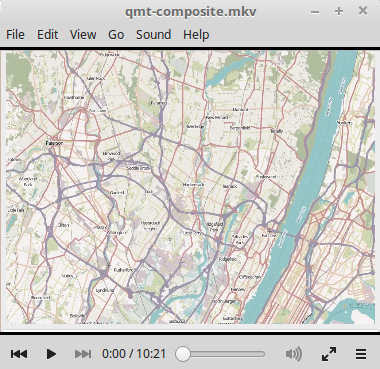
\includegraphics[scale=.3]{pm/qmt-composite.png}\\GIS}}%
% \hspace{10pt}\href{http://www.lingtechsys.com/videos/dhax-composite.mkv}{\parbox{.3\textwidth}{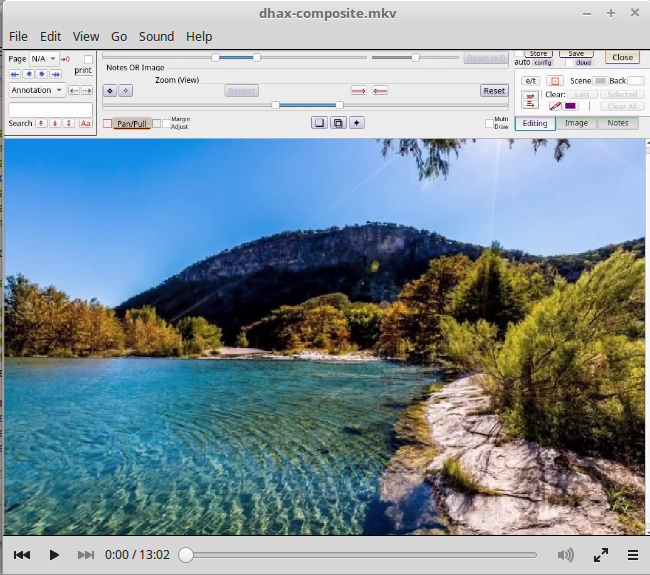
\includegraphics[scale=.255]{pm/dhax-composite.png}\\360\textdegree{} photography}}%
% \hspace{25pt}\href{http://www.lingtechsys.com/videos/xcsd-composite.mkv}{\parbox{.3\textwidth}{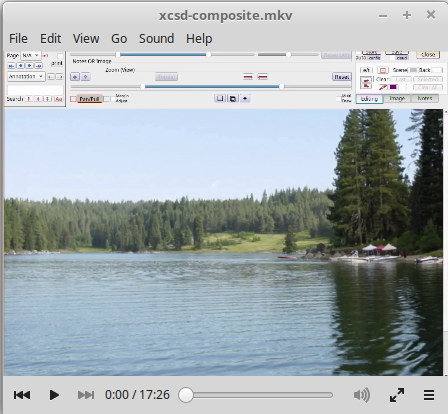
\includegraphics[scale=.35]{pm/xcsd-composite.png}\\Image Processing}}%

}


%\newpage{}





\vspace*{3pt}

\pagestyle{lastpage}
%


%\p{}


\end{document}

% Figure 1  ZoLa compared with a static \PDF{} map
% Figure 2  Merging NYC environment-related classifications 
 %            with WRI and ISI designations
% Figure 3  Custom query windows for accessing E-Designation data
% Figure 4  Customizable basemaps and data-layer overlays
% Figure 5  Managing communications with NYCPlanning \API{}s as part 
 %            of a metro area-wide \API{} integration 




